\chapter{Results}
\section{Quantitative analysis}\label{sec:results}

In what follows there will be four tables per section showing the results of each experiment for four different datasets. CoNSeP and MoNuSAC datasets are available online and are more diverse in content, while DigiPatics breast and DigiPatics lung  are private datasets designed with a more specific goal in mind. Also, at every table the best results will be marked in bold.

\subsection{GNN vs CNN}

This is the main experiment of my thesis. It shows if using graphs improves over not using them. For two out of the three multiclass datasets it do improves, and GNNs also outperform Hovernet in the only binary dataset. Moreover it also lowers the ECE, showing it is not only predicting better but is better calibrated. Nonetheless, the remaining dataset (CoNSeP) poses a question. Why is not working there? Two possible reasons. On the one hand, it is a small dataset with less than 30 images for training and it has 7 classes. This makes the creation of structures quite unusual, cells are more disperse in space not forming groups. And for those that do make groups, there are few samples for the algorithm to learn about it. On the other hand, it may also be that the model is overfitting. It is possible that the probabilities given to the GNN correlate with the target label more in the training that in the test set, making the model learn some patterns that are wrong. Since the other two multiclass datasets have more that 100 images, we deem proper to assume that GNNs start to outperform CNNs when provided with sufficiently enough data. Another remarkable property is that even though GNNs are worse in the CoNSeP dataset overall, they have a lower ECE, meaning they are still better calibrated.

In the datasets that GNNs do improve over CNNs, it is left to discern the real cause why that is happening. When talking to experts, we expected GNNs to be a good fit for the lung dataset but not for the breast one. In the lung dataset they pay special attention to the way cells are grouped together, while in the breast dataset it was not so much the case. So, why does using graphs give better results in both cases? The GNN vs XGBoost and the Void GNN experiments will throw light in this matter.

\begin{table}[ht]
\centering
\caption{Result of the GNN vs CNN experiment.}
\begin{tabular}{c|c|c|c|c|}
  \cline{2-5}
  & Micro $F_1$ score ($\uparrow$) & Macro $F_1$ score ($\uparrow$) & Weighted $F_1$ score ($\uparrow$) & ECE ($\downarrow$) \\ \hline
\multicolumn{1}{|c|}{CNN}  & \textbf{71.11\%} & \textbf{54.06\%} & \textbf{70.39\%} & 0.0680 \\ \hline
\multicolumn{1}{|c|}{GNN}  & 64.44\% & 47.87\% & 61.42\% & \textbf{0.0539} \\ \hline
\end{tabular}
\caption{CoNSeP dataset.}

\vspace{0.5cm}


\begin{tabular}{c|c|c|c|c|}
  \cline{2-5}
  & Micro $F_1$ score ($\uparrow$) & Macro $F_1$ score ($\uparrow$) & Weighted $F_1$ score ($\uparrow$) & ECE ($\downarrow$) \\ \hline
\multicolumn{1}{|c|}{CNN}  & 82.06 \% & 68.76\% & 82.34\% & 0.0774 \\ \hline
\multicolumn{1}{|c|}{GNN}  & \textbf{88.71\%} & \textbf{69.72\%} & \textbf{89.05\%} & \textbf{0.0251}  \\ \hline
\end{tabular}
\caption{MoNuSAC dataset.}

\vspace{0.5cm}

\begin{tabular}{c|c|c|c|c|}
  \cline{2-5}
  & Micro $F_1$ score ($\uparrow$) & Macro $F_1$ score ($\uparrow$) & Weighted $F_1$ score ($\uparrow$) & ECE ($\downarrow$) \\ \hline
\multicolumn{1}{|c|}{CNN}  & 65.12\% & 40.55\% & 66.38\% & 0.3243 \\ \hline
\multicolumn{1}{|c|}{GNN}  & \textbf{70.47\%} & \textbf{42.53\%} & \textbf{71.13\%} & \textbf{0.2501} \\ \hline
\end{tabular}
\caption{DigiPatics breast dataset.}

\vspace{0.5cm}

\begin{tabular}{c|c|c|c|c|c|}
  \cline{2-6}
  & Accuracy ($\uparrow$) & $F_1$ score ($\uparrow$) & ROC AUC ($\uparrow$) & ECE ($\downarrow$) & \%Err ($\downarrow$) \\ \hline
\multicolumn{1}{|c|}{CNN}  & 82.39\% & 57.69\% & 75.20\% & 0.1653 & 11.89\% \\ \hline
\multicolumn{1}{|c|}{GNN}  & \textbf{83.27\%} & \textbf{66.53\%} & \textbf{86.84\%} & \textbf{0.0884} & \textbf{3.52\%} \\ \hline
\end{tabular}
\caption{DigiPatics lung dataset.}
\label{tab:gnn-cnn}
\end{table}

\newpage
\subsection{GNN vs XGBoost}

In the first experiment it was shown that GNNs outperform CNNs in most of the scenarios. But why? Is it due to the relations among cells or due to stacking another classifier on top of the CNN? In the former we should expect GNN to also outperform a node-only method like XGBoost. If it is the latter, then XGBoost should win. As we can see here, the answer is not crystal clear. In some cases it is better to use GNNs and in others it is not. In order to further elucidate when is the case in advance to training the models, the qualitative analysis will help give some insight. Looking at individual images will provide some keys about when graphs are a good fit. Moreover, we find that for those datasets where GNN perform better, in the Void GNN experiment the models trained without probabilities also perform better. While for those that XGBoost is the winner here, the models with probabilities are the winner there. Showcasing that for MoNuSAC and Digipatic lung datasets, the graph structure is indeed important and the performance boost is not due to stacking a classifier on top. This is also consistent with our prior knowledge of the breast dataset. We didn't expect graphs to be a good fit because they indeed aren't. Their performance boost is because of the overall model being a stack classifier.

\begin{table}[ht]
    \centering
    \caption{Result of the GNN vs XGBoost experiment.}
    \begin{tabular}{c|c|c|c|c|}
  \cline{2-5}
  & Micro $F_1$ score ($\uparrow$) & Macro $F_1$ score ($\uparrow$) & Weighted $F_1$ score ($\uparrow$) & ECE ($\downarrow$) \\ \hline
\multicolumn{1}{|c|}{XGB}  & \textbf{71.54\%} & \textbf{51.64\%} & \textbf{69.87\%} & \textbf{0.0320} \\ \hline
\multicolumn{1}{|c|}{GNN}  & 64.44\% & 47.87\% & 61.42\% & 0.0539  \\ \hline
\end{tabular}
\caption{CoNSeP dataset.}

\vspace{0.5cm}

\begin{tabular}{c|c|c|c|c|}
  \cline{2-5}
  & Micro $F_1$ score ($\uparrow$) & Macro $F_1$ score ($\uparrow$) & Weighted $F_1$ score ($\uparrow$) & ECE ($\downarrow$) \\ \hline
\multicolumn{1}{|c|}{XGB}  & 85.23\% & \textbf{76.09\%} & 85.20\% & 0.0449 \\ \hline
\multicolumn{1}{|c|}{GNN}  & \textbf{88.71\%} & 69.72\% & \textbf{89.05\%} & \textbf{0.0251} \\ \hline
\end{tabular}
\caption{MoNuSAC dataset.}

\vspace{0.5cm}

\begin{tabular}{c|c|c|c|c|}
  \cline{2-5}
  & Micro $F_1$ score ($\uparrow$) & Macro $F_1$ score ($\uparrow$) & Weighted $F_1$ score ($\uparrow$) & ECE ($\downarrow$)  \\ \hline
\multicolumn{1}{|c|}{XGB}  & \textbf{78.51\%} & \textbf{47.36\%} & \textbf{79.78\%} & 0.2502   \\ \hline
\multicolumn{1}{|c|}{GNN}  & 70.47\% & 42.53\% & 71.13\% & \textbf{0.2501}   \\ \hline
\end{tabular}
\caption{DigiPatics breast dataset.}

\vspace{0.5cm}

\begin{tabular}{c|c|c|c|c|c|}
  \cline{2-6}
  & Accuracy ($\uparrow$) & $F_1$ score ($\uparrow$) & ROC AUC ($\uparrow$) & ECE ($\downarrow$) & \%Err ($\downarrow$) \\ \hline
\multicolumn{1}{|c|}{XGB}  & \textbf{83.77\%} & 62.64\% & 84.20\% & 0.1007 & 7.85\% \\ \hline
\multicolumn{1}{|c|}{GNN}  & 83.27\% & \textbf{66.53\%} & \textbf{86.84\%} & \textbf{0.0884} & \textbf{3.52\%} \\ \hline
\end{tabular}
\caption{DigiPatics lung dataset.}
    \label{tab:gnn-xgb}
\end{table}

\newpage
\subsection{Scaling CNNs}

Deleting last layer weights and retraining can give better performance, as shown below in \autoref{tab:consep-scaling}. 270FT performs better than 270 and 518FT better than 518 for the CoNSeP dataset. This aligns perfectly with the results from \cite{zhou2022fortuitous}. They observe that reinitialising weights and retraining can boost performance. In our setup this translates to fine-tuning a model in the same dataset it was pretrained. Also, you may have noticed that the metrics for 518FT are slightly different than those in the GNN vs CNN experiment even though they are the same model. That is because we trained the same model twice converging to slightly different checkpoints. I provide both metrics to demonstrate that the ordering is the same using either of both metrics, thus proving training is sufficiently stable.

Same result is obtained for MoNuSAC dataset. Fine-tuning the checkpoint trained on CoNSeP helps obtain better results when applied as initialisation for the models trained on MoNuSAC dataset which comes from a totally different distribution. The features learned by the encoder seems to generalise well to this other dataset. However, the results in the breast dataset differ from the ones in the CoNSeP and MoNuSAC datasets. In that case using a pretrained checkpoint didn't perform well at neither resolution. This may be because the local minima found for the CoNSeP dataset is far away from the nearest minima in the DigiPatics breast dataset, making a random initialisation a better method. Another reason may be that the breast dataset has a colour distribution very different that the others, probably because it used a different staining method.

Another remarkable fact is that using a field of view of 518 pixels instead of 270 gives better metrics no matter the initialisation nor the dataset, except for lung. We would have liked to further try a bigger field of view. But training the 518 models required more than 20 GB of GPU VRAM. Scaling to 1030x1030 images would require near 80 GB of GPU VRAM, which is only feasible using A100 or H100, which cost more than 10000€. Using CPU offloading was also not an option since that technique trades memory for time, typically increasing by 100 the time required. The models required around 4 hours to train. This means one experiment may take up to 2 weeks with a bigger field of view, which is clearly prohibitive. With our resources, 518 was the maximum we could achieve.

The lung case is quite strange for two reasons. First, because a smaller field of view gives better results while on the other datasets it doesn't. And second, because in previous experiments we made when the labels were not reviewed by an expert revealed exactly the opposite pattern. The DigiPatics lung dataset went through an iterative process until it arrived at the state it is here. The scaling experiment consistently gave better results for 518FT at all the steps except at the last one, when the labels were all reviewed by an expert. Although we still use the 518FT backbone for the GNN, it doesn't invalidate the point since the two stages are independent. We are just showing that adding a graph neural network on top improves, that is independent from improving the segmentation model.

\begin{table}[ht]
    \centering
    \caption{Result of the Scaling CNNs experiment.}
    \begin{tabular}{c|c|c|c|}
  \cline{2-4}
  & Micro $F_1$ score ($\uparrow$) & Macro $F_1$ score ($\uparrow$) & Weighted $F_1$ score ($\uparrow$) \\ \hline
\multicolumn{1}{|c|}{270}  & 54.20\% & 36.21\% & 54.62\% \\ \hline
\multicolumn{1}{|c|}{270FT}  & 66.73\% & 49.01\% & 65.96\% \\ \hline
\multicolumn{1}{|c|}{518}  & 56.75\% & 37.76\% & 59.45\% \\ \hline
\multicolumn{1}{|c|}{518FT}  & \textbf{71.02\%} & \textbf{53.83\%} & \textbf{70.52\%} \\ \hline
\end{tabular}
\caption{CoNSeP dataset.}
\label{tab:consep-scaling}


\vspace{0.5cm}

\begin{tabular}{c|c|c|c|}
  \cline{2-4}
  & Micro $F_1$ score ($\uparrow$) & Macro $F_1$ score ($\uparrow$) & Weighted $F_1$ score ($\uparrow$)  \\ \hline
\multicolumn{1}{|c|}{270}  & 76.46\% & 56.20\% & 77.04\% \\ \hline
\multicolumn{1}{|c|}{270FT}  & 77.97\% & 62.84\% & 77.93\% \\ \hline
\multicolumn{1}{|c|}{518}  & 78.57\% & 58.64\% & 79.61\% \\ \hline
\multicolumn{1}{|c|}{518FT}  & \textbf{82.02\%} & \textbf{70.40\%} & \textbf{82.09\%} \\ \hline
\end{tabular}
\caption{MoNuSAC dataset.}

\vspace{0.5cm}

\begin{tabular}{c|c|c|c|c|}
  \cline{2-4}
  & Micro $F_1$ score ($\uparrow$) & Macro $F_1$ score ($\uparrow$) & Weighted $F_1$ score ($\uparrow$) \\ \hline
\multicolumn{1}{|c|}{270}  & 70.04\% & 38.22\% & 68.43\%  \\ \hline
\multicolumn{1}{|c|}{270FT}  & 48.55\% & 21.57\% & 34.44\% \\ \hline
\multicolumn{1}{|c|}{518}  & \textbf{72.36\%} & \textbf{45.64\%} & \textbf{75.80\%} \\ \hline
\multicolumn{1}{|c|}{518FT}  & 68.78\% & 43.27\% & 71.58\% \\ \hline
\end{tabular}
\caption{DigiPatics breast dataset.}

\vspace{0.5cm}

\begin{tabular}{c|c|c|c|}
  \cline{2-4}
  & Accuracy ($\uparrow$) & $F_1$ score ($\uparrow$) & ROC AUC ($\uparrow$)  \\ \hline
\multicolumn{1}{|c|}{270}  & 78.77\% & 67.17\% & 79.00\% \\ \hline
\multicolumn{1}{|c|}{270FT}  & \textbf{85.46\%} & \textbf{71.65\%} & \textbf{79.90\%} \\ \hline
\multicolumn{1}{|c|}{518}  & 81.07\% & 56.16\% & 69.73\% \\ \hline
\multicolumn{1}{|c|}{518FT}  & 82.22\% & 57.01\% & 70.13\% \\ \hline
\end{tabular}
\caption{DigiPatics lung dataset.}
    \label{tab:scaling}
\end{table}

\newpage
\subsection{Void GNNs}

Another way of seeing if the good performance of graphs is due to the information in the edges or in the attributes of the nodes, is to train the graphs models with and without the attributes. If there is no performance difference, then edges are relevant. Otherwise, it is less relevant. Moreover, there is a set of attributes that depends on the layers behind, the probabilities. To discern if GNNs are working cause they are stacked above or because there is a graph structure we also train the models with and without the probabilities. We observe that in the datasets that XGBoost did not outperform GNNs the GNN trained with no information about the prior probability given by Hovernet do in fact perform better than the model with those probabilities. However, in the two datasets that XGBoost did give better results we can see that using probabilities gives a benefit over using other types of features. This tells us that MoNuSAC and DigiPatics lung datasets have more structure than CoNSeP and DigiPatics breast datasets. In DigiPatics breast GNNs gave better results than CNN but it was due to stacking. For DigiPatics lung it was because the graph is indeed a good way of modelling the problem. 

Another conclusion that derives from this tables is that some kind of features are needed, no matter how simple they are. Training the graph networks without any feature at all gave very poor results. It also resulted in a more unstable training in general. Providing the model with some information about the individual cells is crucial for the proper functioning of the method.

\begin{table}[ht]
    \centering
    \caption{Result of the Void GNNs experiment.}
    \resizebox{0.9\textwidth}{!}{\begin{tabular}{c|c|c|c|c|}
  \cline{2-5}
  & Micro $F_1$ score ($\uparrow$) & Macro $F_1$ score ($\uparrow$) & Weighted $F_1$ score ($\uparrow$) & ECE ($\downarrow$) \\ \hline
\multicolumn{1}{|c|}{Full}  & 64.44\% & \textbf{47.87\%} & 61.42\% & 0.0539  \\ \hline
\multicolumn{1}{|c|}{Probabilities}  & \textbf{64.93\%} & 47.37\% & \textbf{61.63\%} & \textbf{0.0494} \\ \hline
\multicolumn{1}{|c|}{Morphological}  & 52.11\% & 29.42\% & 48.19\% & 0.0582 \\ \hline
\multicolumn{1}{|c|}{Void}  & 29.88\% & 8.08\% & 15.78\% & 0.0742 \\ \hline
\end{tabular}}
\caption{CoNSeP dataset.}

\vspace{0.2cm}

\resizebox{0.9\textwidth}{!}{\begin{tabular}{c|c|c|c|c|}
  \cline{2-5}
  & Micro $F_1$ score ($\uparrow$) & Macro $F_1$ score ($\uparrow$) & Weighted $F_1$ score ($\uparrow$) & ECE ($\downarrow$) \\ \hline
\multicolumn{1}{|c|}{Full}  & 88.71\% & 69.72\% & 89.05\% & \textbf{0.0251}  \\ \hline
\multicolumn{1}{|c|}{Probabilities}  & 82.59\% & \textbf{73.43\%} & 82.60\% & 0.0784 \\ \hline
\multicolumn{1}{|c|}{Morphological}  & \textbf{92.01\%} & 69.83\% & \textbf{92.02\%} & 0.0405 \\ \hline
\multicolumn{1}{|c|}{Void}  & 53.61\% & 26.65\% & 52.20\% & 0.0580 \\ \hline
\end{tabular}}
\caption{MoNuSAC dataset.}

\vspace{0.2cm}

\resizebox{0.9\textwidth}{!}{\begin{tabular}{c|c|c|c|c|}
  \cline{2-5}
  & Micro $F_1$ score ($\uparrow$) & Macro $F_1$ score ($\uparrow$) & Weighted $F_1$ score ($\uparrow$) & ECE ($\downarrow$) \\ \hline
\multicolumn{1}{|c|}{Full}  & \textbf{70.47\%} & \textbf{42.53\%} & \textbf{71.13\%} & 0.2501  \\ \hline
\multicolumn{1}{|c|}{Probabilities}  & 67.94\% & 40.83\% & 68.91\% & 0.2666 \\ \hline
\multicolumn{1}{|c|}{Morphological}  & 63.05\% & 30.48\% & 61.26\% & 0.2676 \\ \hline
\multicolumn{1}{|c|}{Void}  & 36.91\% & 11.86\% & 24.96\% & \textbf{0.2413} \\ \hline
\end{tabular}}
\caption{DigiPatics breast dataset.}

\vspace{0.2cm}

\resizebox{0.9\textwidth}{!}{\begin{tabular}{c|c|c|c|c|c|}
  \cline{2-6}
  & Accuracy ($\uparrow$) & $F_1$ score ($\uparrow$) & ROC AUC ($\uparrow$) & ECE ($\downarrow$) & \%Err ($\downarrow$) \\ \hline
\multicolumn{1}{|c|}{Full}  & 83.27\% & 66.53\% & 86.84\% & 0.0884 & 3.52\% \\ \hline
\multicolumn{1}{|c|}{Probabilities}  & 82.87\% & 63.10\% & 87.26\% & 0.0470\% & 7.08\% \\ \hline
\multicolumn{1}{|c|}{Morphological}  & \textbf{83.81\%} & \textbf{70.18\%} & \textbf{88.88\%} & \textbf{0.0431\%} & \textbf{0.78\%} \\ \hline
\multicolumn{1}{|c|}{Void}  & 73.24\% & 0.00\% & 54.66\% & 0.1250 & 26.76\% \\ \hline
\end{tabular}}
\caption{DigiPatics lung dataset.}
    \label{tab:void-gnn}
\end{table}

\newpage
\subsection{CNNs metrics in detail}

In all the experiments above I provided metrics only for 1-1 matchings of cells. That is a fair way of comparing CNN to GNN since GNN can only improve predictions on 1-1 matchings. However, it does not show the full picture. The CNN can miss cells or predict cells that do not exist. For that reason I here provide the same metrics as above but adding one extra class: the background. It never has true positives, only false positives and false negatives. Thus, it will almost always be worse than the metrics above given. For a counter example on when it is not worse, look at the next paragraph. The bigger the gap, the more cells it is missing or incorrectly predicting. Nevertheless, such gap does not alter any of the conclusions. In this project we did not try to narrow this gap because we consider the classification problem to be inherently more difficult than the segmentation problem. We believe improving the segmentation problem is simply a matter of more data and bigger models. If you think about it, you can detect cells without formal knowledge, it is just a matter of geometry and color. But recognising where are the tumours located? That requires more than 10 years of training to humans, and even in that case experts still have doubts. Therefore we directed our efforts toward improving the classification, not the segmentation.

You may have noticed that in the DigiPatics breast dataset the macro $F_1$ score did not worsen when adding the background. It seems counterintuitive since we are adding a class with no true positives, only false positives and false negatives. But, the key to why this happens is purely technical. This is the global confusion matrix for the test set in the DigiPatics breast dataset:

\[
\begin{bmatrix}
0 & 95 & 151 & 116 & 9 & 425 \\
26 & 100 & 14 & 1 & 0 & 64 \\
518 & 752 & 1136 & 819 & 17 & 445 \\
25 & 6.0 & 54 & 336 & 28 & 5 \\
0 & 0 & 0 & 0 & 0 & 0 \\
509 & 48 & 18 & 3 & 1 & 2672
\end{bmatrix}
\]

\noindent Why is this matrix problematic? Well, there is one class which does not appear at all in the ground truth. The reason why this causes the problem is because the two macro $F_1$ scores are computed differently. The "With Background" metrics are computed using the confusion matrix and a custom function I designed. The "Without Background" metrics are computed using pairs of labels and the sklearn f1\_score function. Both functions are coded properly, that is not the problem. But in my implementation of the metric, I coded a function that estimates the number of classes based on the classes with support in the ground truth, and also ignoring the zero class. However, the sklearn function estimates the number of classes as the class with the maximum label. This is making one metric being divided by 4 and another being divided by 5. If we adjust the sklearn given metric to consider 4 classes instead of 5 we get a macro $F_1$ score of $50.69\%$ which is bigger than $44.56\%$ as expected. The reason I don't adjust this metric in the other tables is because the GNN methods are also evaluated using the sklearn function so the comparison is fair as it is. I just left the metrics below unchanged to showcase how a simple decision in design of an algorithm or method can affect the final conclusions, even creating mathematically impossible situations.

\begin{table}[ht]
\centering
\caption{Hovernet evaluated with and without background in four different datasets.}
\begin{tabular}{c|c|c|c|}
  \cline{2-4}
  & Micro $F_1$ score & Macro $F_1$ score & Weighted $F_1$ score \\ \hline
\multicolumn{1}{|c|}{With Background}  & 48.38\% & 49.58\% & 57.84\% \\ \hline
\multicolumn{1}{|c|}{Without Background}  & \textbf{71.11\%} & \textbf{54.06\%} & \textbf{70.39\%} \\ \hline
\end{tabular}
\caption{CoNSeP dataset.}

\vspace{0.5cm}


\begin{tabular}{c|c|c|c|}
  \cline{2-4}
  & Micro $F_1$ score & Macro $F_1$ score & Weighted $F_1$ score \\ \hline
\multicolumn{1}{|c|}{With Background}  & 53.29\% & 43.95\% & 67.67\% \\ \hline
\multicolumn{1}{|c|}{Without Background}  & \textbf{82.06\%} & \textbf{68.76\%} & \textbf{82.34\%} \\ \hline
\end{tabular}
\caption{MoNuSAC dataset.}

\vspace{0.5cm}

\begin{tabular}{c|c|c|c|}
  \cline{2-4}
  & Micro $F_1$ score & Macro $F_1$ score & Weighted $F_1$ score \\ \hline
\multicolumn{1}{|c|}{With Background}  & 50.57\% & \textbf{44.56\%} & 57.89\% \\ \hline
\multicolumn{1}{|c|}{Without Background}  & \textbf{65.12\%} & 40.55\% & \textbf{66.38\%}  \\ \hline
\end{tabular}
\caption{DigiPatics breast dataset.}

\vspace{0.5cm}

\begin{tabular}{c|c|c|c|c|c|c|c|}
  \cline{2-7}
  & Accuracy & $F_1$ score & ROC AUC & Micro $F_1$ & Macro $F_1$ & Weighted $F_1$ \\ \hline
\multicolumn{1}{|c|}{With Background}  & NA & NA & NA & 66.12\% & 66.06\% & 72.11\% \\ \hline
\multicolumn{1}{|c|}{Without Background}  & 82.39\% & 57.69\% & 75.20\% & NA & NA & NA \\ \hline
\end{tabular}
\caption{DigiPatics lung dataset.}
\label{tab:cnn-vis}
\end{table}

\newpage
\section{Qualitative analysis}

In this section I will be providing insights as to why and when graph neural networks are a good regularizer. The overall effect of using GNNs can be described as finding groups. In some cases it is a good approach in others it isn't, it depends on the data. Throughout this sections I will be referring to all the classes by their colours. They all have a more profound meaning, like epithelial or inflammatory or tumoural. But for simplicity I will just refer to them by the colour they are painted with.

\subsection{CoNSeP}

This dataset is the smallest of all four which makes a model with higher inductive bias like Hovernet perform better. Graphs are a more general structure, and that means they require more data to function properly. As a first example look at \autoref{fig:consep-qual1}. Hovernet tries to identify some of the green cells while the graph convolution just consider everything to be a big group. However, Hovernet also misclassifies some cells as blue or yellow when they are not, which is something the GCN does not do. In this aspect, and as will be seen with more examples, GCN normally play safe and assign the class with more cells as the main class of the group. GCNs do not typically try to find outliers which is something Hovernet does but sometimes, as in this case, it fails. Graph attention on the other hand may focus on smaller groups. In this case, GAT has managed to properly identify a small green nest of cells, just missing one of the cells in that nest. 

\begin{figure}[H]
  \centering
  \begin{subfigure}[b]{0.45\textwidth}
    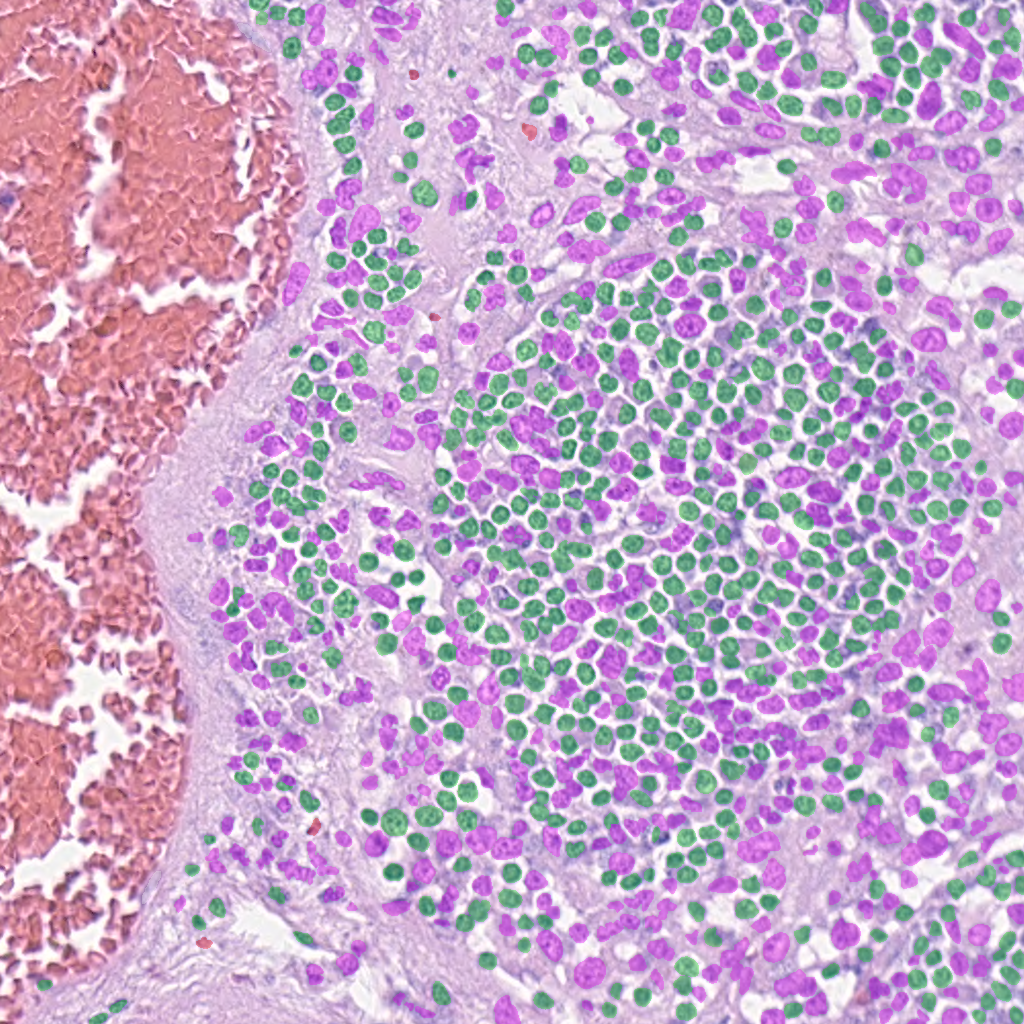
\includegraphics[width=\textwidth]{imgs/qual/consep/gt1.overlay.png}
    \caption{GT}
    \label{fig:consep-gt1}
  \end{subfigure}
  \hfill
  \begin{subfigure}[b]{0.45\textwidth}
    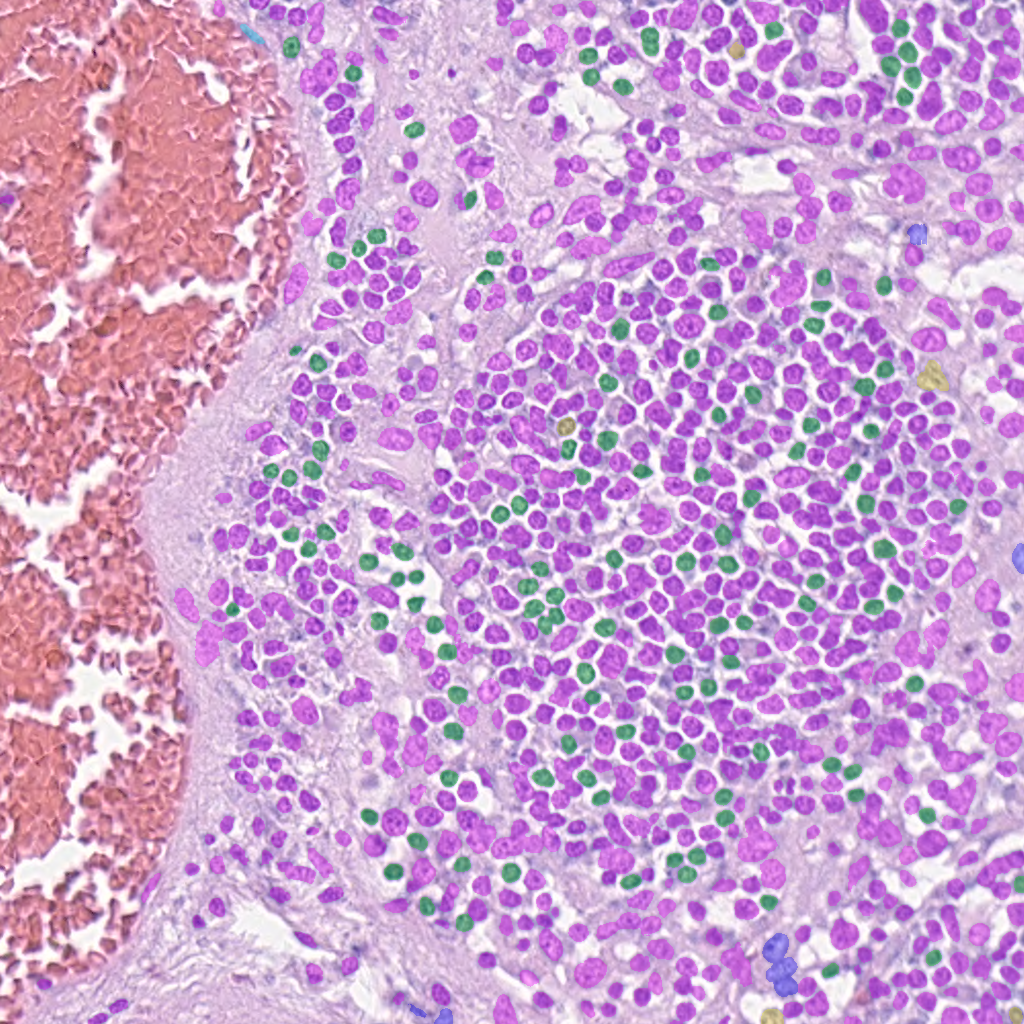
\includegraphics[width=\textwidth]{imgs/qual/consep/hov1.png}
    \caption{Hovernet}
    \label{fig:consep-hov1}
  \end{subfigure}
  \\
  \begin{subfigure}[b]{0.45\textwidth}
    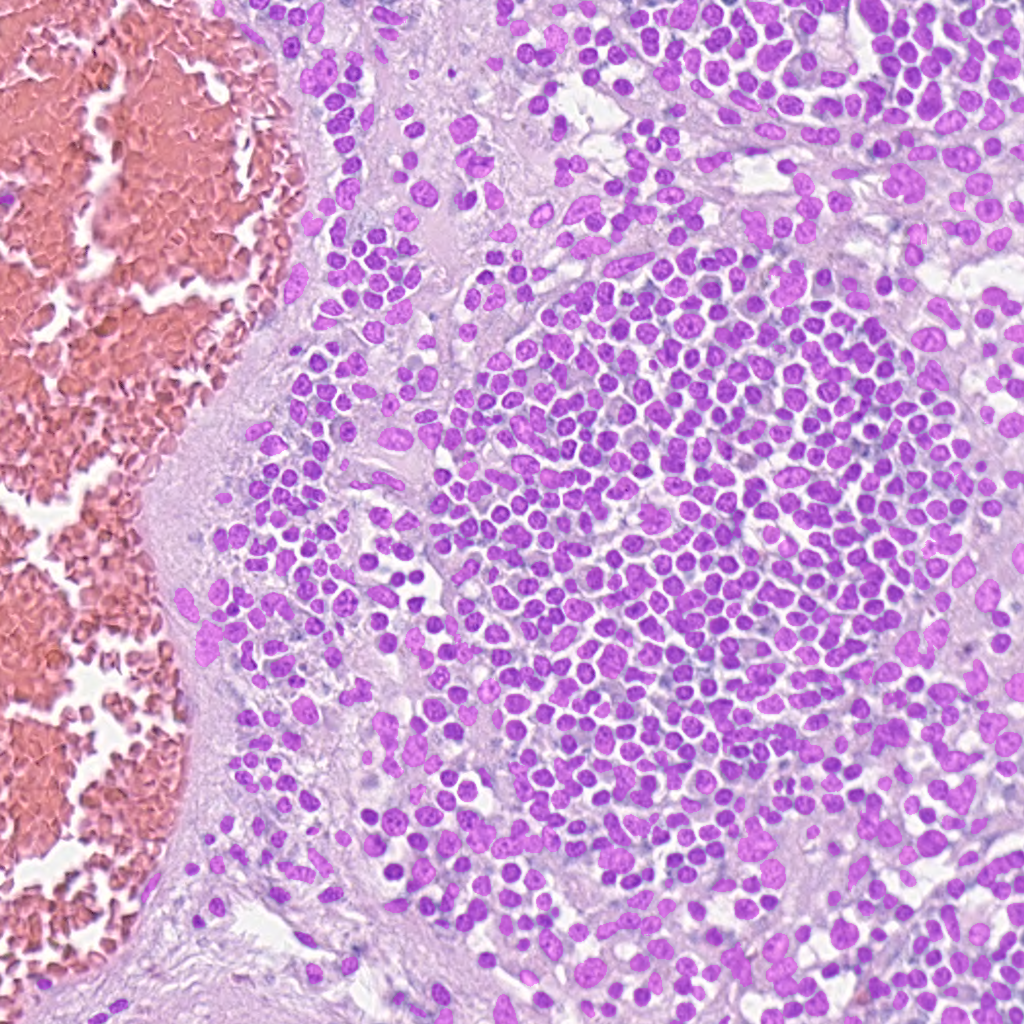
\includegraphics[width=\textwidth]{imgs/qual/consep/gcn-full1.png}
    \caption{GCN}
    \label{fig:consep-gcn1}
  \end{subfigure}
  \hfill
  \begin{subfigure}[b]{0.45\textwidth}
    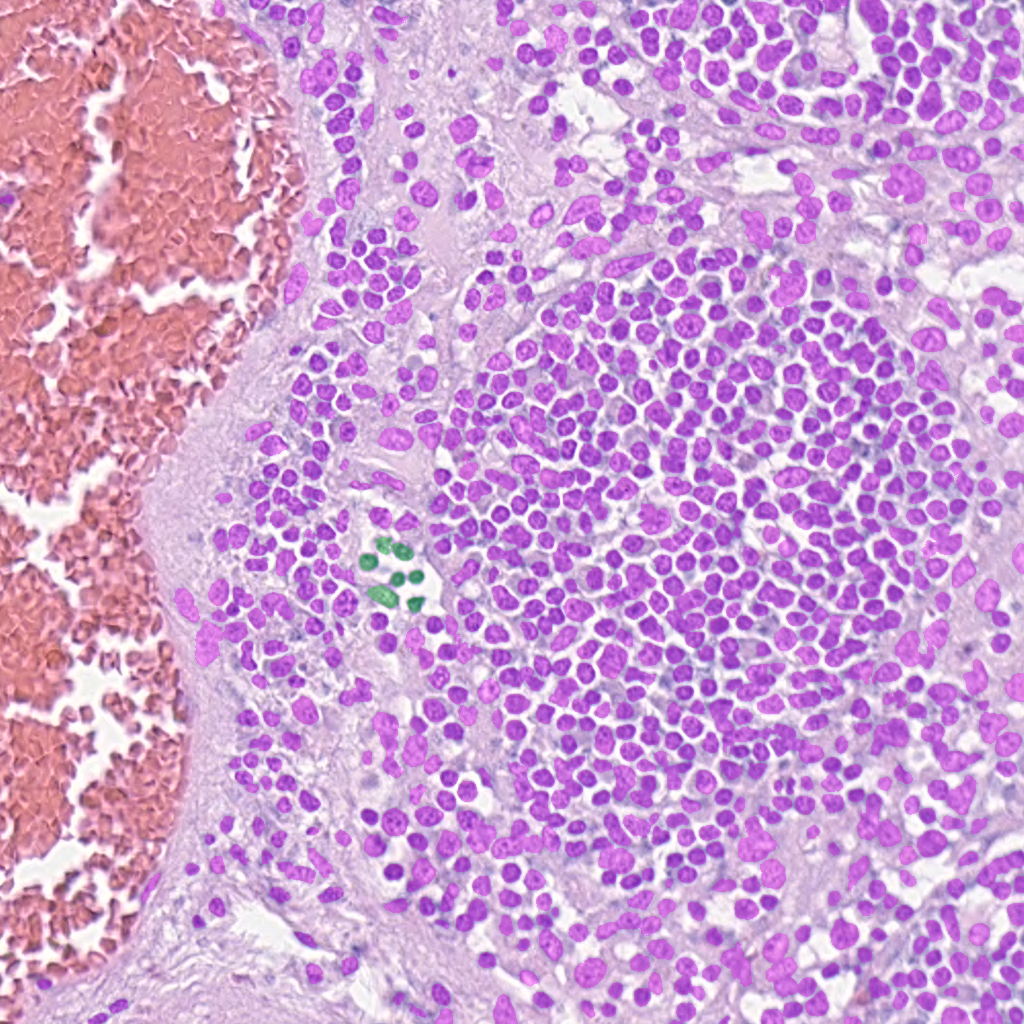
\includegraphics[width=\textwidth]{imgs/qual/consep/gat-full1.png}
    \caption{GAT}
    \label{fig:consep-gat1}
  \end{subfigure}
  \caption{Comparison of the predictions of Hovernet, graph convolution and graph attention methods.}
  \label{fig:consep-qual1}
\end{figure}

To illustrate how diverse is this concrete dataset, I will show another example where the sizes of the cells are different, the labels are different, and the way the cells are structured is also different. This example shows how difficult this dataset is. With so many classes, the number of possible ways of arranging cells is very high. Making less than 30 images not enough for the graph to learn something useful. 

\begin{figure}[H]
  \centering
  \begin{subfigure}[b]{0.45\textwidth}
    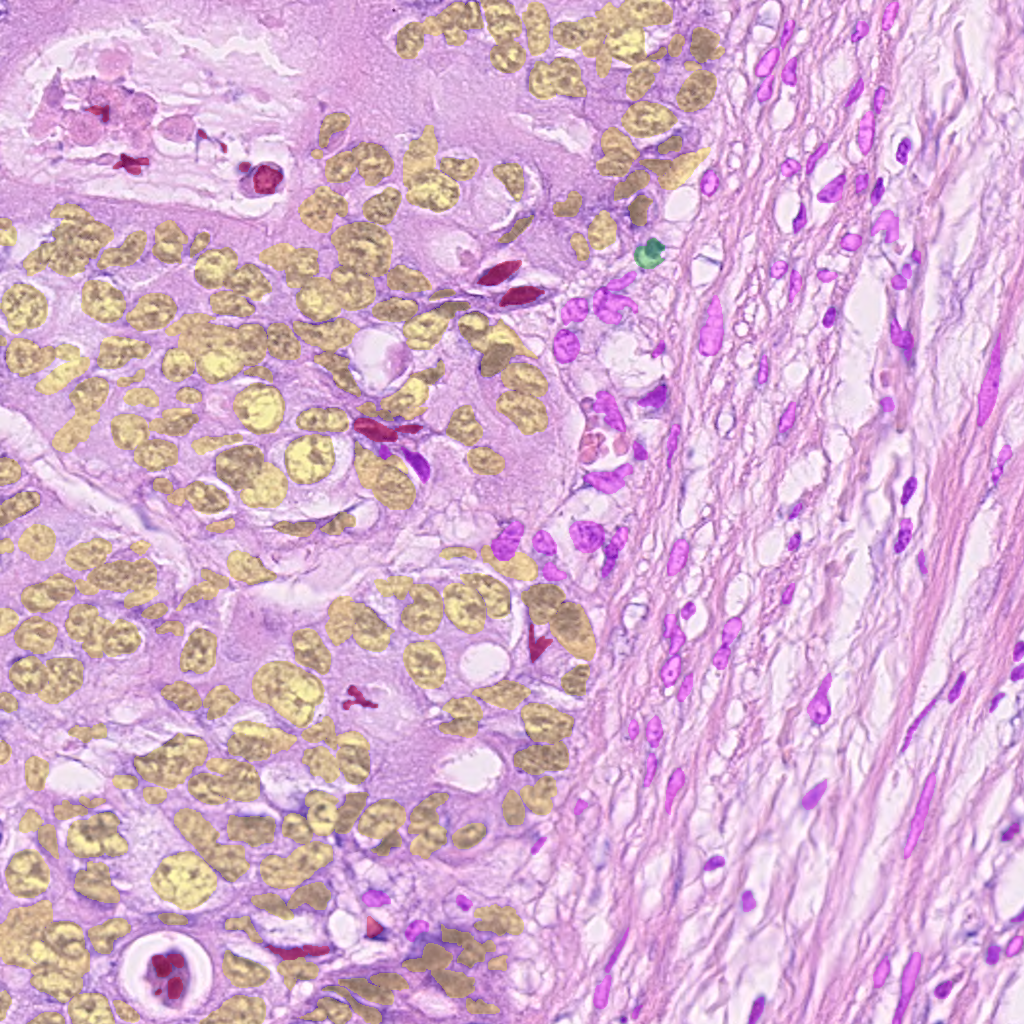
\includegraphics[width=\textwidth]{imgs/qual/consep/gt2.overlay.png}
    \caption{GT}
    \label{fig:consep-gt2}
  \end{subfigure}
  \hfill
  \begin{subfigure}[b]{0.45\textwidth}
    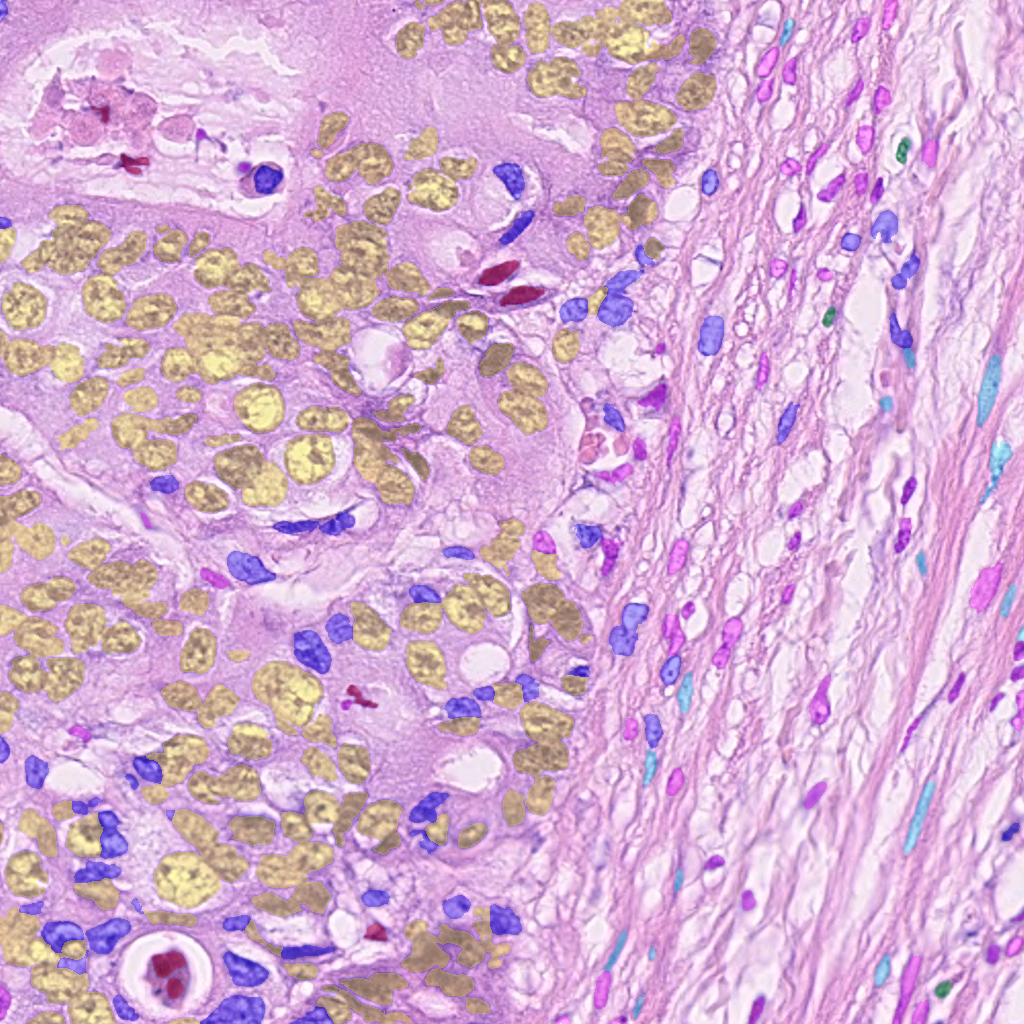
\includegraphics[width=\textwidth]{imgs/qual/consep/hov2.png}
    \caption{Hovernet}
    \label{fig:consep-hov2}
  \end{subfigure}
  \\
  \begin{subfigure}[b]{0.45\textwidth}
    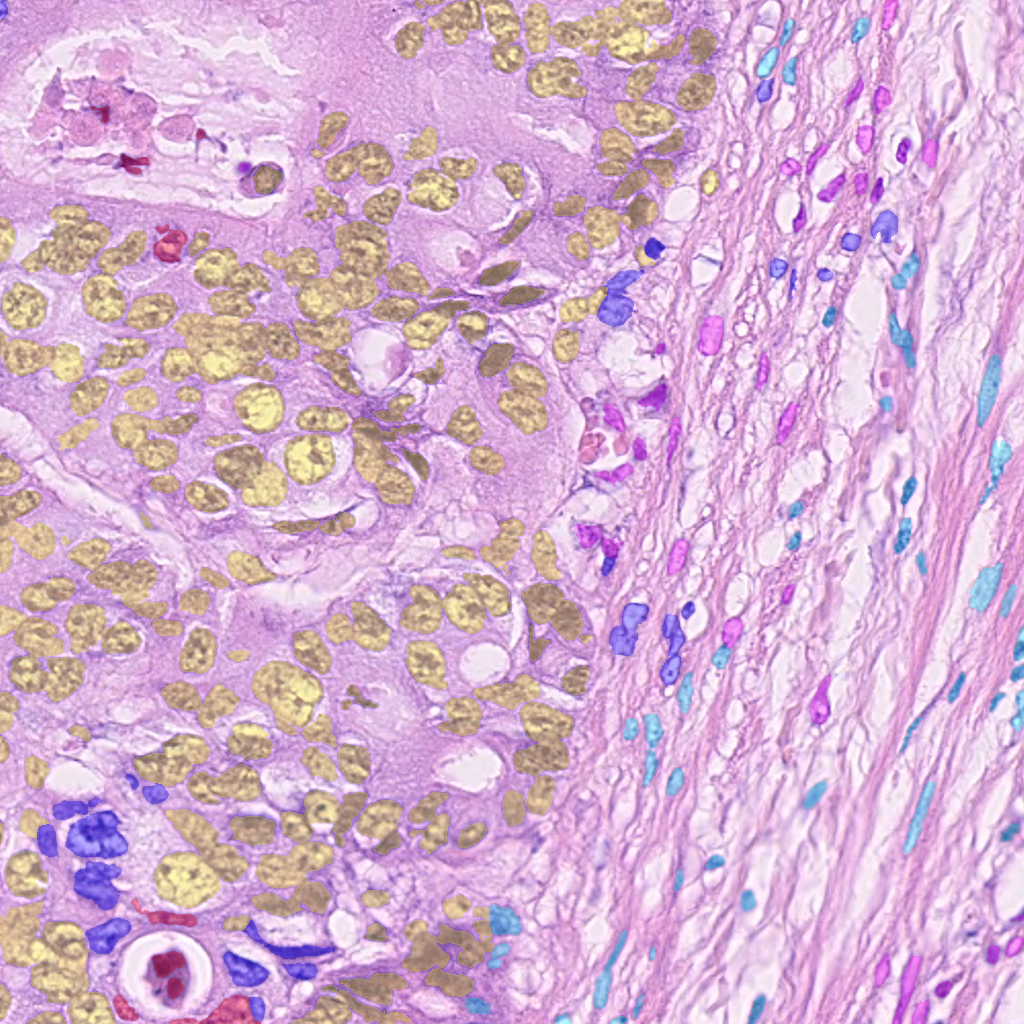
\includegraphics[width=\textwidth]{imgs/qual/consep/gcn-full2.png}
    \caption{GCN}
    \label{fig:consep-gcn2}
  \end{subfigure}
  \hfill
  \begin{subfigure}[b]{0.45\textwidth}
    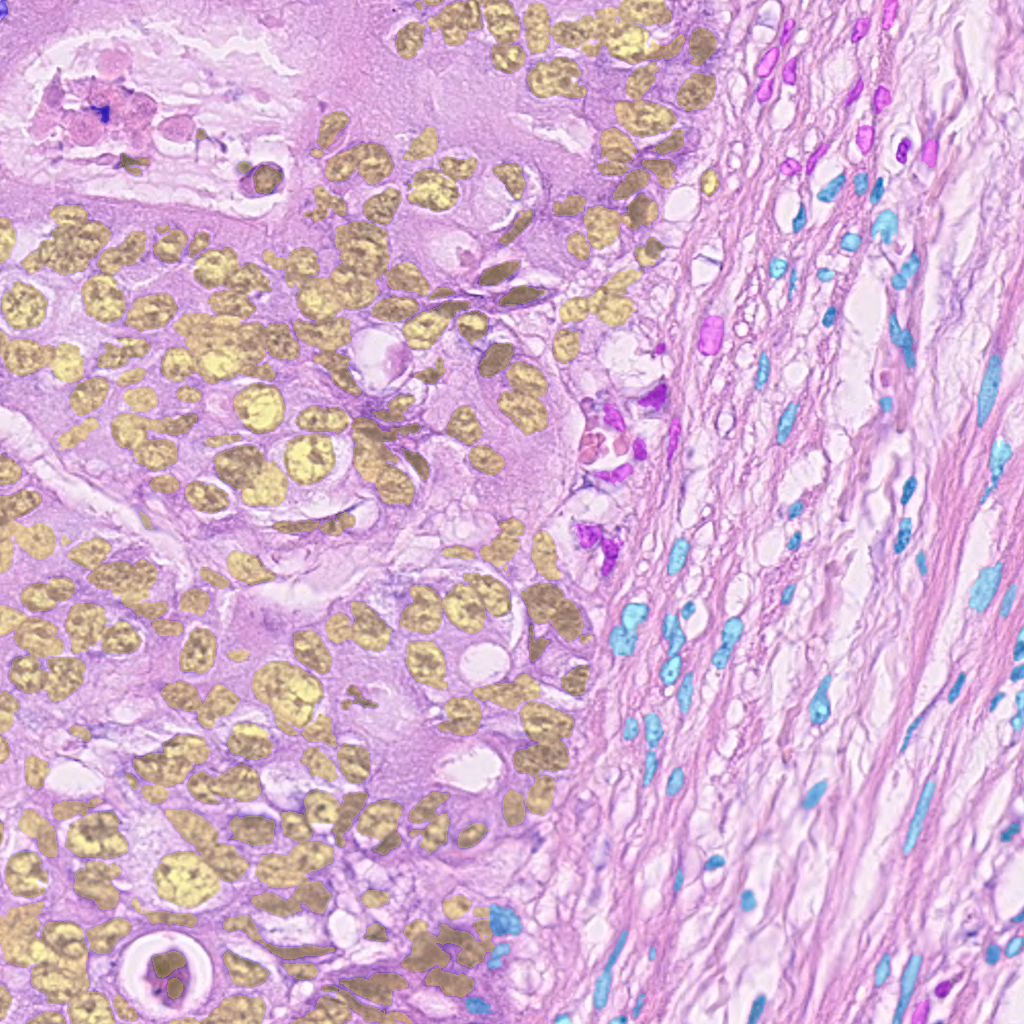
\includegraphics[width=\textwidth]{imgs/qual/consep/no-morph2.png}
    \caption{Probabilities only}
    \label{fig:consep-no-morph2}
  \end{subfigure}
  \\
  \begin{subfigure}[b]{0.45\textwidth}
    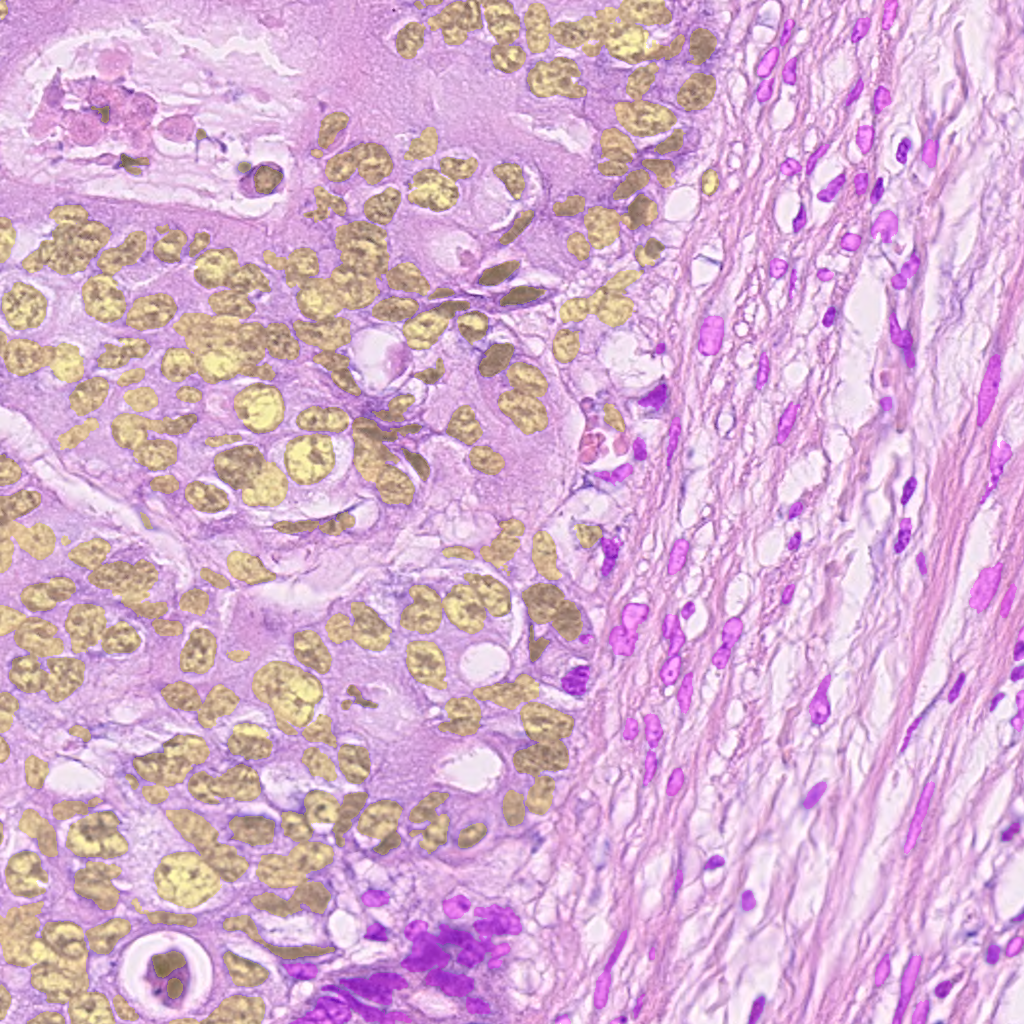
\includegraphics[width=\textwidth]{imgs/qual/consep/no-prior2.png}
    \caption{Morphological features only}
    \label{fig:consep-no-prior2}
  \end{subfigure}
  \hfill
  \begin{subfigure}[b]{0.45\textwidth}
    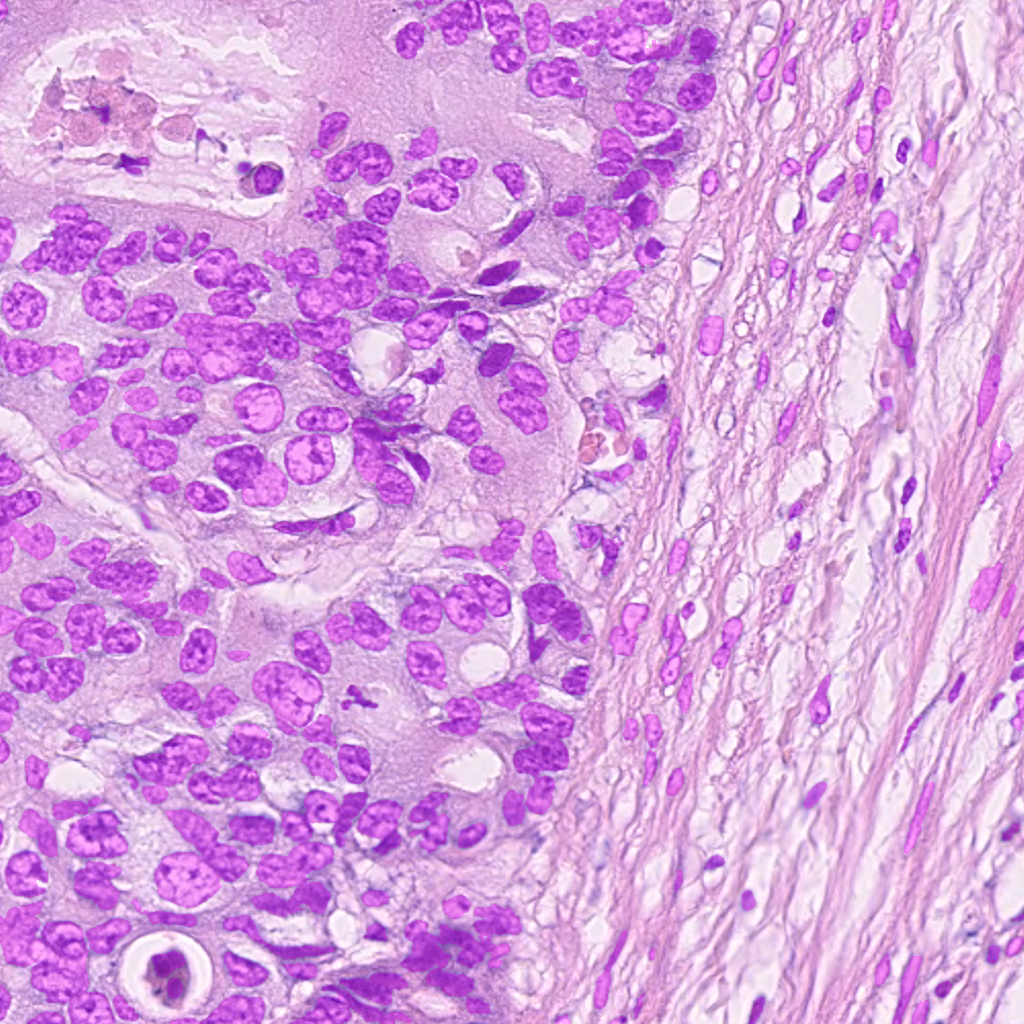
\includegraphics[width=\textwidth]{imgs/qual/consep/void2.png}
    \caption{Void}
    \label{fig:consep-void2}
  \end{subfigure}
  \caption{Illustration of the behaviour of the different models.}
  \label{fig:consep-qual2}
\end{figure}

\newpage

In \autoref{fig:consep-qual2} we can see that Hovernet misses some of the magenta cells and classifies them as blue. Here, the effect of the GCN is positive in some aspects and negative in others. The positive side is that it recovers most of the yellow cells thanks to considering them as a whole. The negative aspect is that it expands the cyan cells which were initially misclassified by Hovernet. This is a common pattern. Since the GNN operates using the probabilities from Hovernet, it can propagate the errors from it. As further proof of that look at the same example, but now look at the output from the models trained without the probabilities of Hovernet and trained only with those probabilities. The model that was trained only with probabilities further propagates the cyan group while the model trained without them did not produce any cyan cells at all. There is a trade-off when using Hovernet probabilities. It can help fix groups where Hovernet misclassified a few of the inner cells. But relying too much on Hovernet probabilities can worsen the results. When using just morphological features, the GNN is more independent from Hovernet which in this case was beneficial. Nonetheless, using no features at all is a bad idea. In this specific example the model trained only with the graph but no features classified everything as magenta, wrongly forgetting the yellow cells. Visually it is quite clear that the yellow cells and the magenta ones are a separate group, but if you just consider nodes in a graph, without indicating the area or the perimeter, there is not enough information to detect two groups in this image.

To end with the analysis of this dataset, I will display another image where cells of different types are mixed together. In \autoref{fig:consep-qual3} we can see how Hovernet predicts a more diverse set of cells than the GCN. It has yellow cells which are not surrounded by other yellow cells, it also has cyan, magenta and blue. In contrast, the GCN has mostly predicted the cyan as the dominant class. The effect of using GNNs is visible again. Hovernet takes risk and predicts lonely cells, cells with no neighbour of the same class. GNNs create neighbourhoods of cells. In this case neither of them are really a good fit since Hovernet predicts many classes that are not real and the GCN cannot really discern the mix of cyan and magenta that is in the middle of the image and predicts the whole middle group as cyan.

\begin{figure}[H]
    \centering
    \begin{subfigure}[b]{0.3\textwidth}
    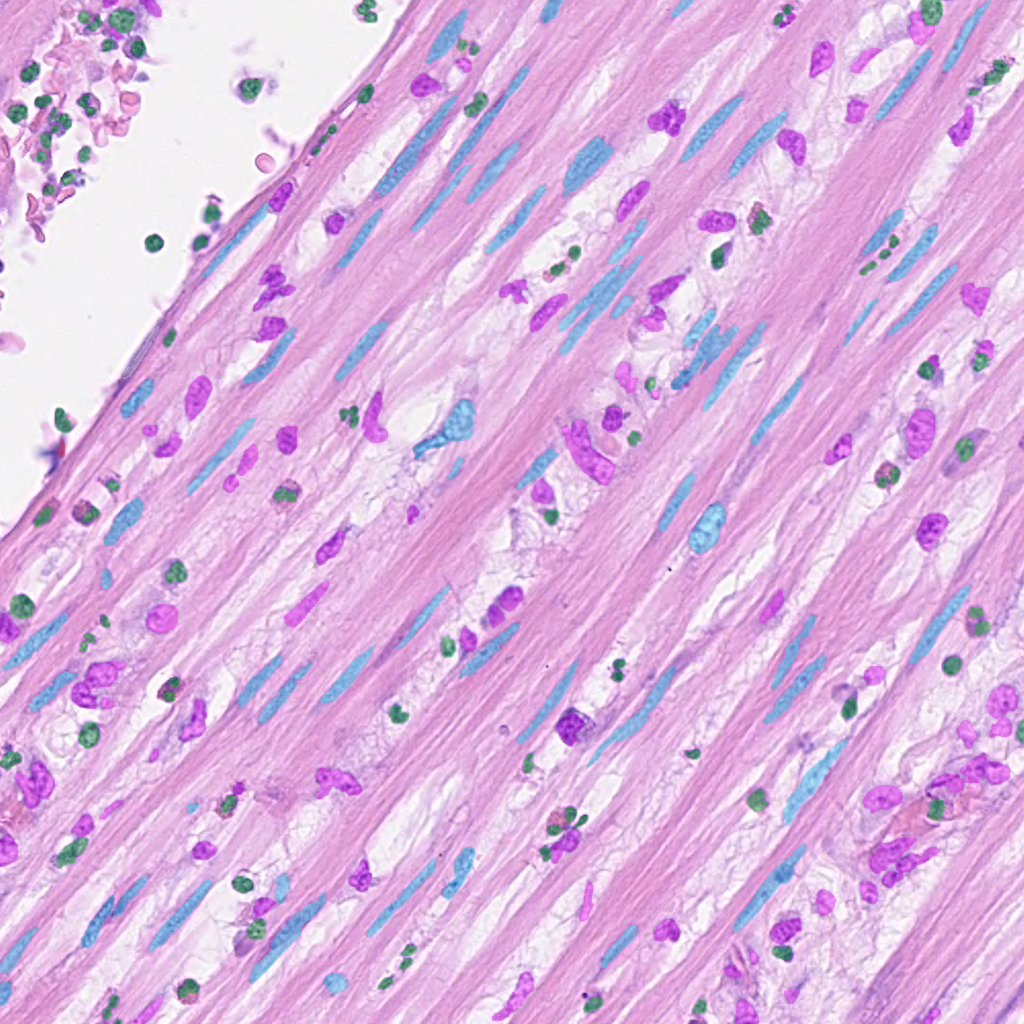
\includegraphics[width=\textwidth]{imgs/qual/consep/gt3.overlay.png}
    \caption{GT}
    \label{fig:consep-gt2}
  \end{subfigure}
  \begin{subfigure}[b]{0.3\textwidth}
    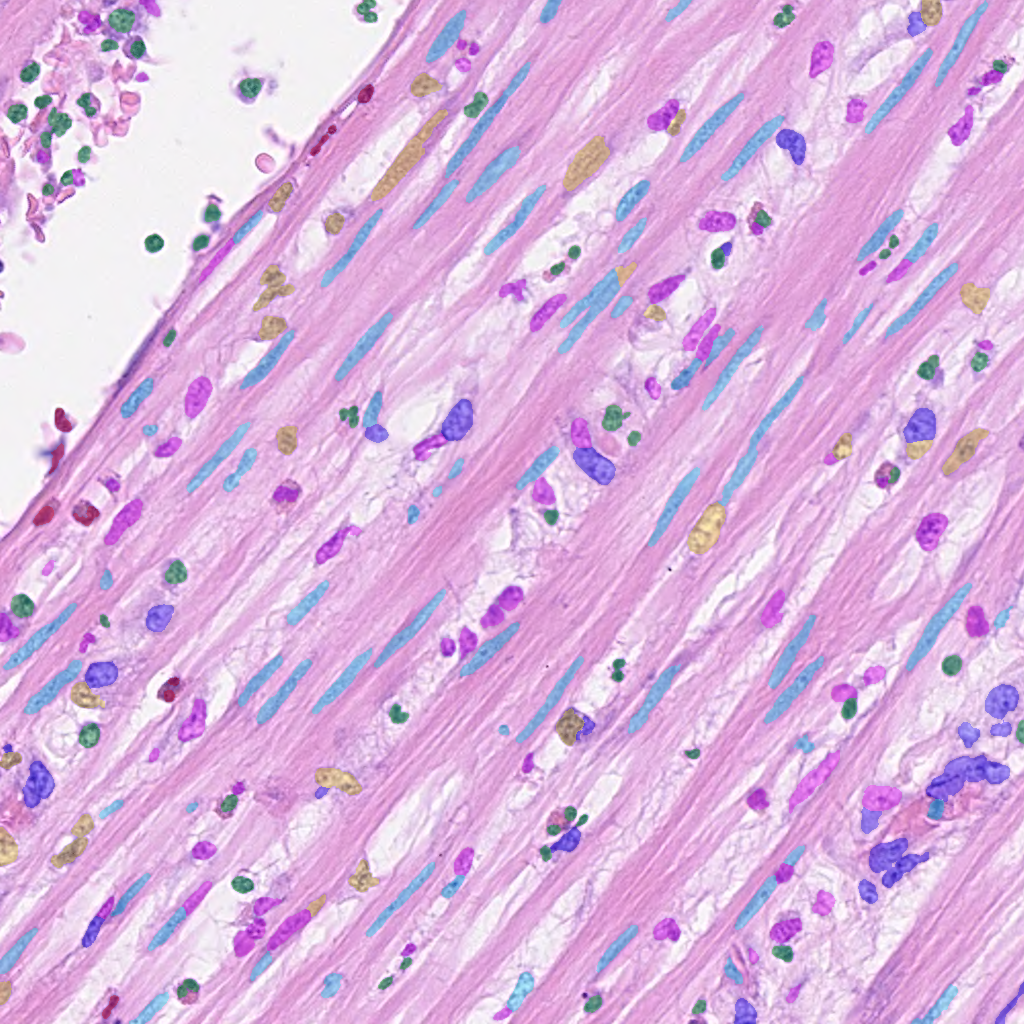
\includegraphics[width=\textwidth]{imgs/qual/consep/hov3.png}
    \caption{Hovernet}
    \label{fig:consep-hov2}
  \end{subfigure}
  \begin{subfigure}[b]{0.3\textwidth}
    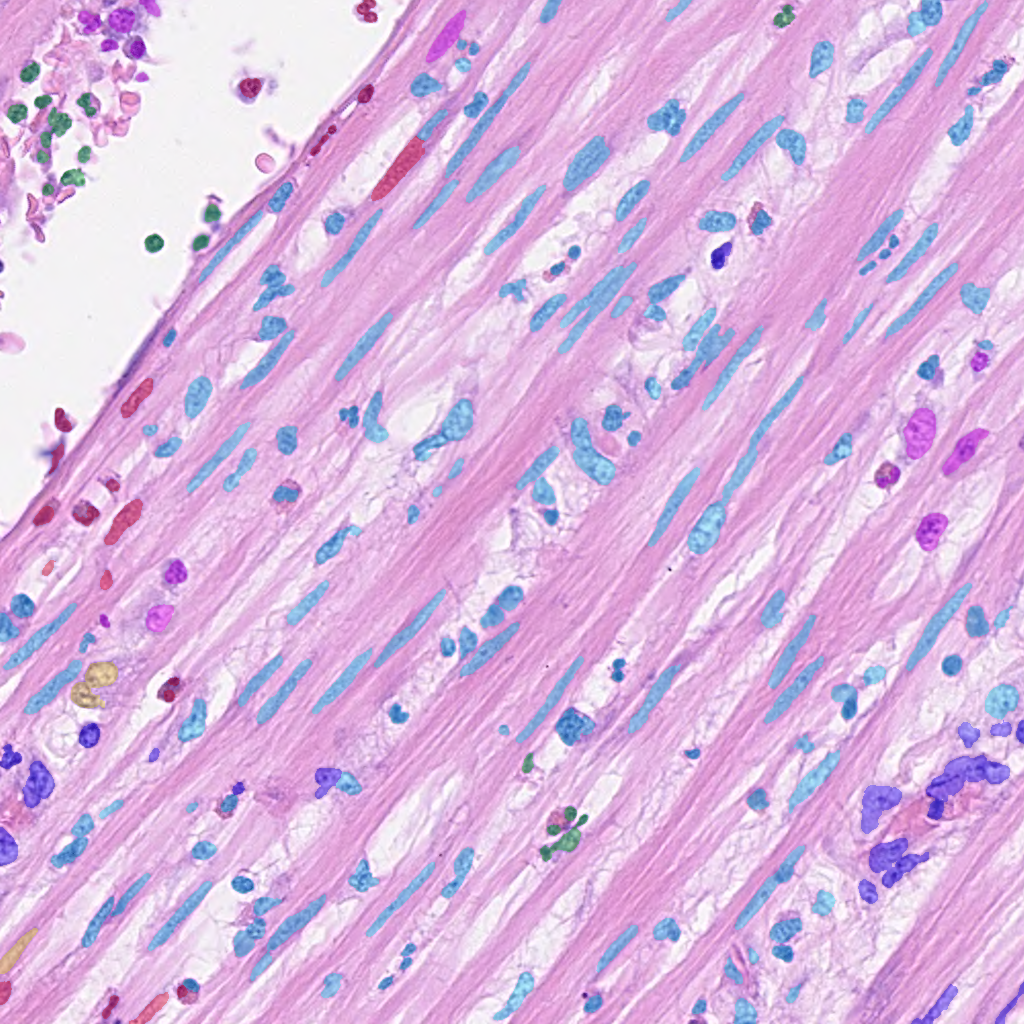
\includegraphics[width=\textwidth]{imgs/qual/consep/gcn-full3.png}
    \caption{GCN}
    \label{fig:consep-gcn2}
  \end{subfigure}
    \caption{Last example of CoNSeP database. It mixes different cell types which makes it difficult for the GNN to work properly.}
    \label{fig:consep-qual3}
\end{figure}

\newpage
\subsection{MoNuSAC}

In previous sections I have stated that this dataset was a good example of where the graph neural networks are a good fit. With the CoNSeP dataset we have seen that those models tend to group cell togethers. When there is a mix of different classes it works poorly. In \autoref{fig:monusac-ex} we can see three examples out of this dataset which are exactly the opposite. They contain well defined groups. It is difficult to appreciate but in the image on the left there are two well defined groups, one green and one red and in the image at the left there are also blue cells close to each other. Many of the images in this dataset are like the one in the middle, with only one class in the whole image. Having this setup it is expected to see Hovernet misclassify some cells since it is not considering the image as a whole while the GNNs solve that problem by merging everything into big groups.

\begin{figure}[H]
    \centering
    \begin{subfigure}[b]{0.3\textwidth}
    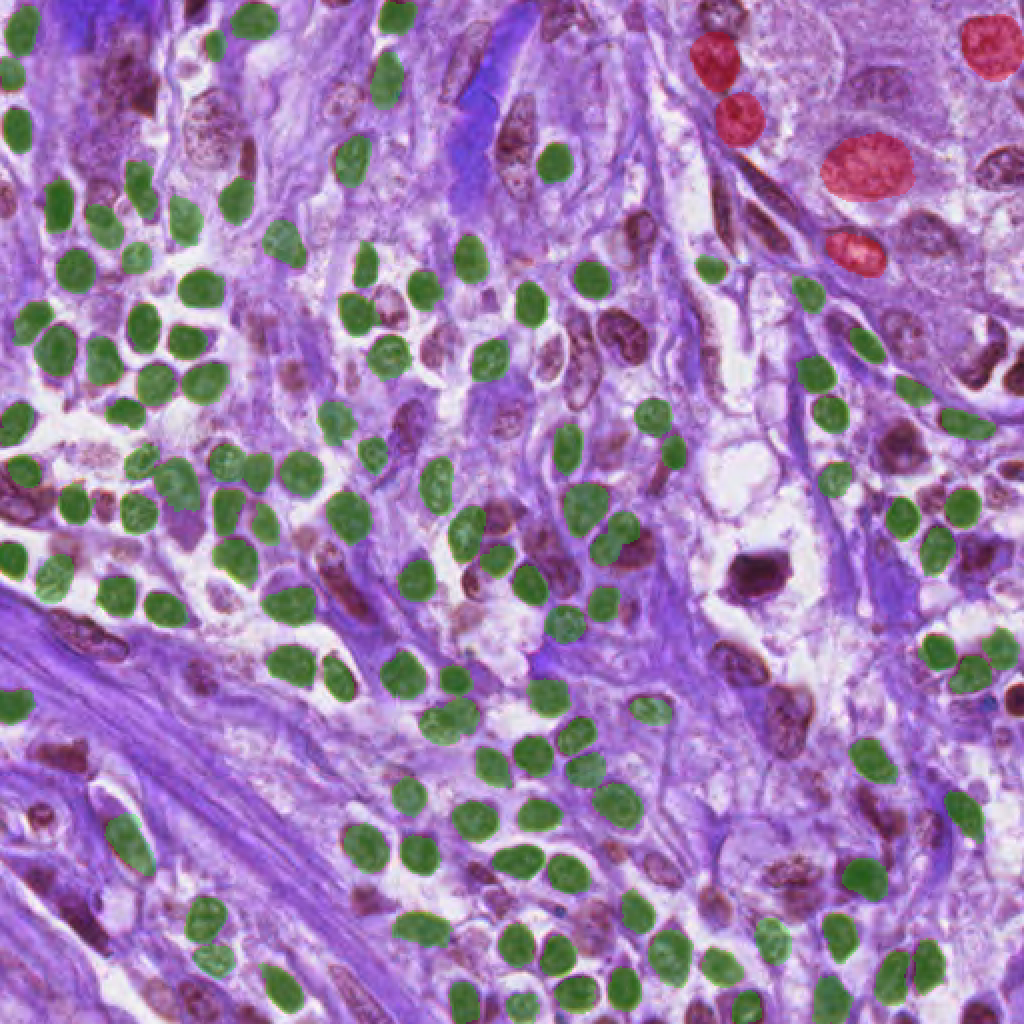
\includegraphics[width=\textwidth]{imgs/qual/monusac/gt1.overlay.png}
    \label{fig:monusac-gt1}
  \end{subfigure}
  \begin{subfigure}[b]{0.3\textwidth}
    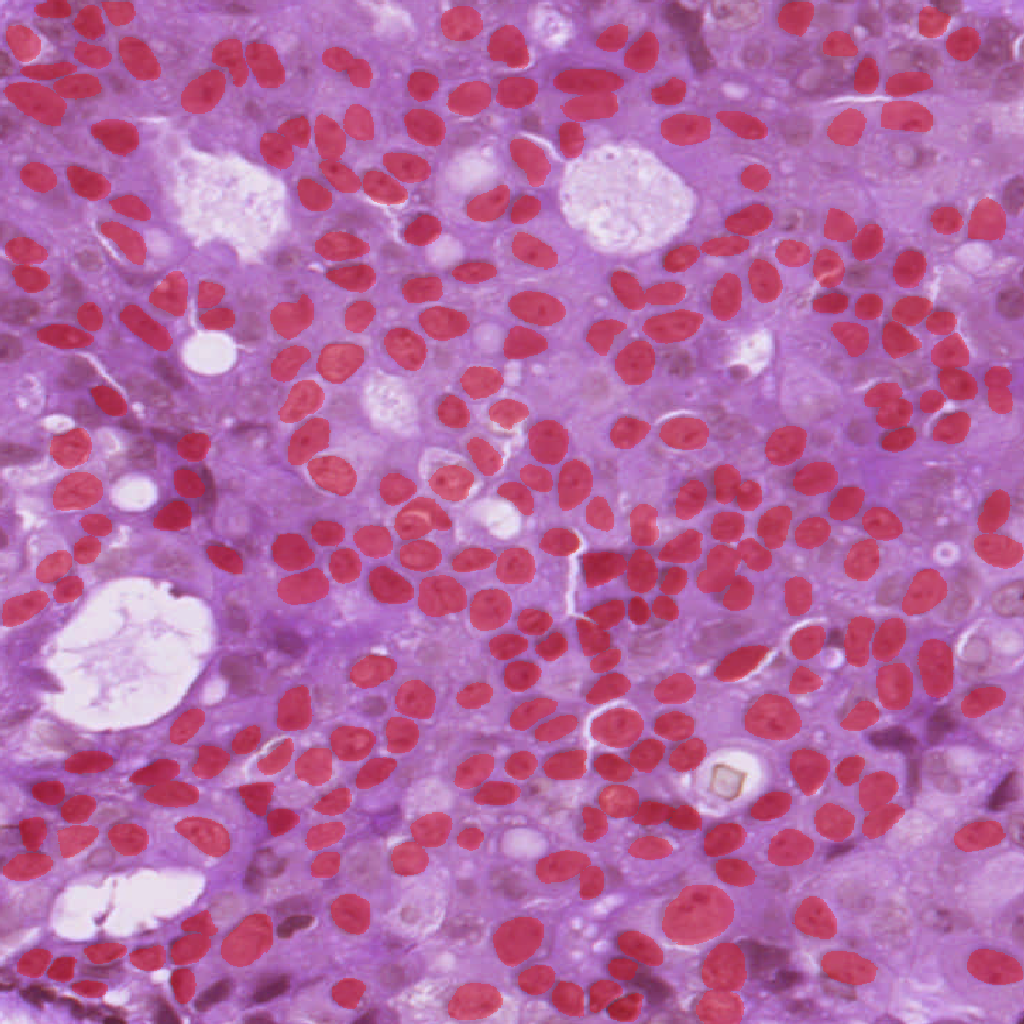
\includegraphics[width=\textwidth]{imgs/qual/monusac/gt2.overlay.png}
    \label{fig:monusac-gt2}
  \end{subfigure}
  \begin{subfigure}[b]{0.3\textwidth}
    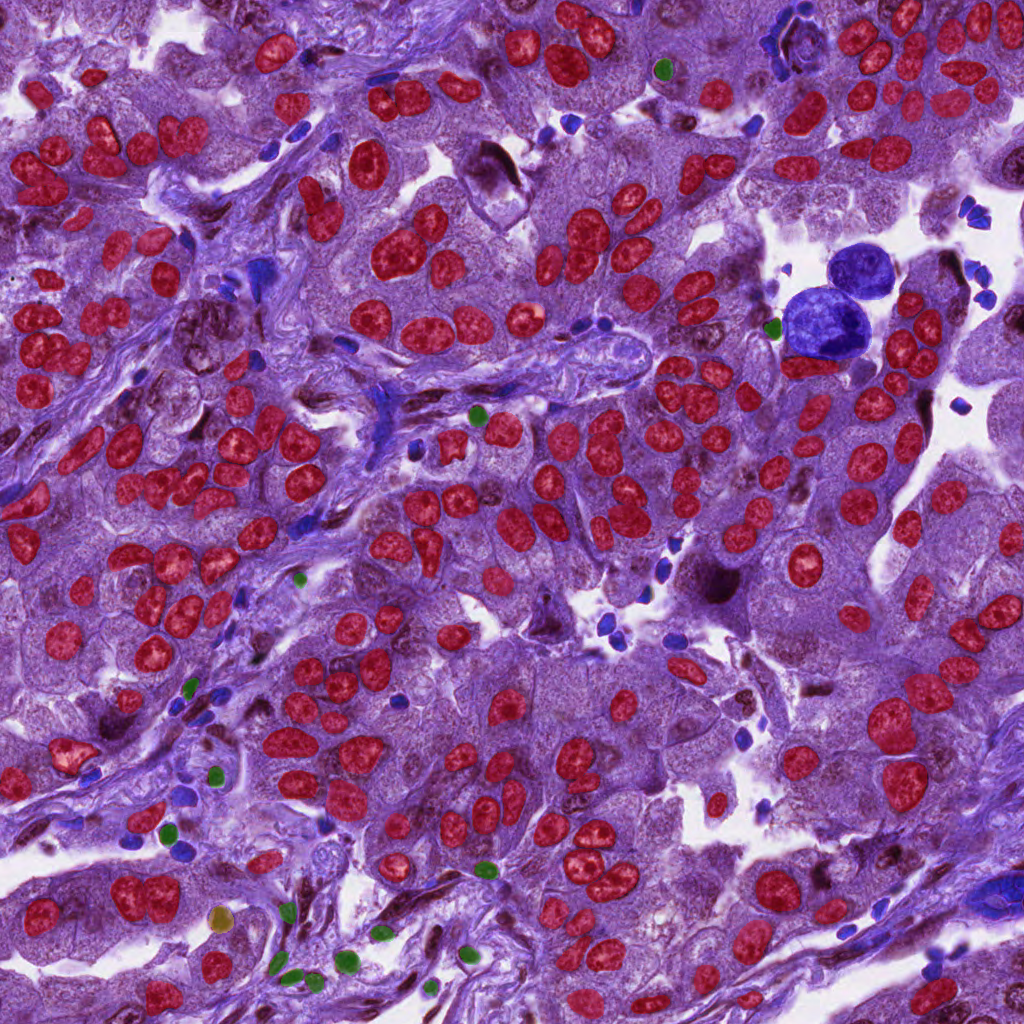
\includegraphics[width=\textwidth]{imgs/qual/monusac/gt3.overlay.png}
    \label{fig:monusac-gt3}
  \end{subfigure}
    \caption{Three examples with their ground truth overlayed on top.}
    \label{fig:monusac-ex}
\end{figure}

Let's dive into the details of what every model predicted with the image on the left. Same as what happened in CoNSeP, here in \autoref{fig:monusac-qual1} the Hovernet randomly misclassifies some green cells into red cells. The graph network that was trained only with Hovernet probabilities believes it and so it creates three nests. The green in the middle, the red at the top right and the red at the bottom left grouping and merging the result from the Hovernet. The network trained with morphological features is more correct in that the group at the bottom left is correctly classified as green while preserving the red group at the top right. The GCN trained with everything is confused and so it simply predicts everything as green. Finally, the GCN that only sees the graph and no features at all behaves a bit unpredictably, creating another group of red cells at the bottom right and at the top left.

Similar conclusions can be drawn with the result obtained from the image on the right of \autoref{fig:monusac-ex}. The output is on \autoref{fig:monusac-qual3}. The result with the remaining image at the center of \autoref{fig:monusac-ex} is less informative. In there all the models correctly predicted every cell as red. Even though Hovernet sometimes randomly misclassifies little cells, there are cases like the one in the middle of \autoref{fig:monusac-ex} that everything is correctly classified. When there is only one group to classify, the graph networks will be as right as Hovernet. After all, they are using the probabilities as inputs and creating clusters of cells. If there is only one cluster, there is not much work to do.

\begin{figure}[H]
  \centering
  \begin{subfigure}[b]{0.45\textwidth}
    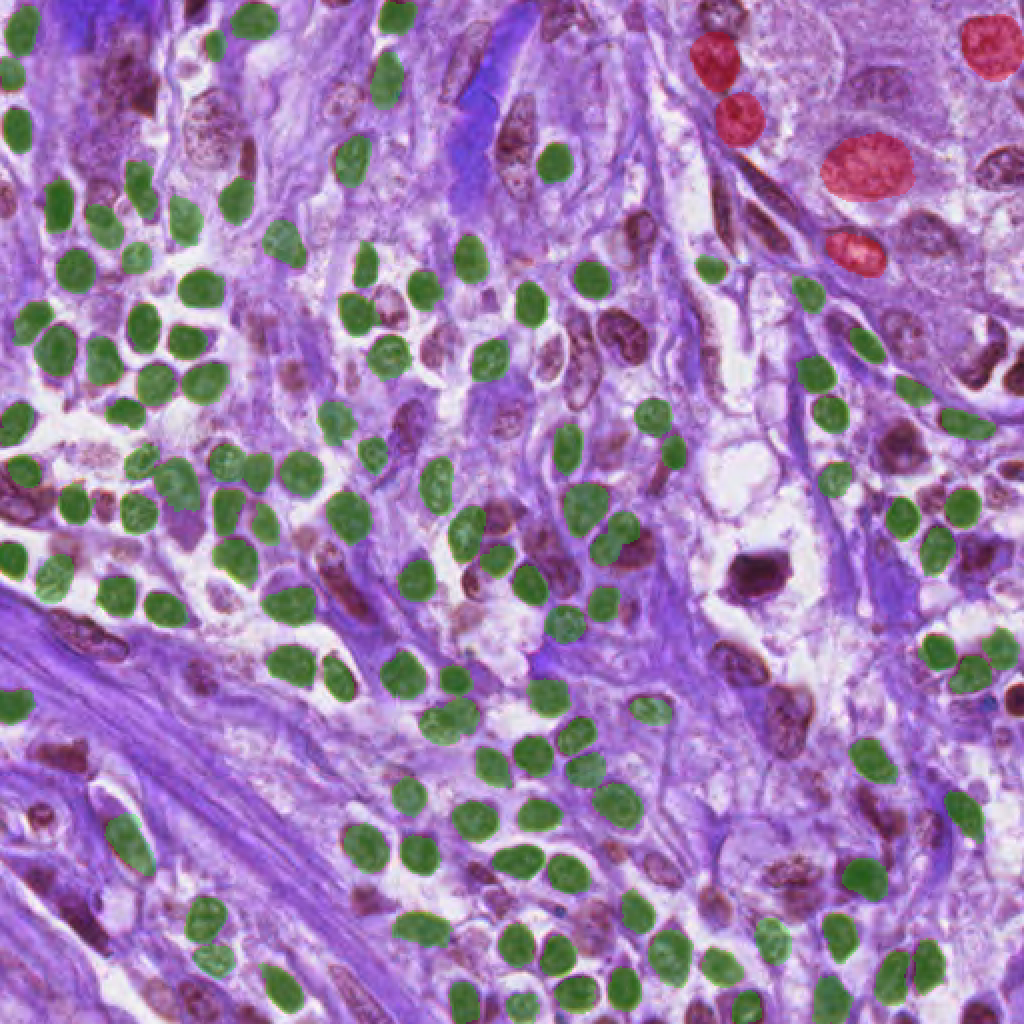
\includegraphics[width=\textwidth]{imgs/qual/monusac/gt1.overlay.png}
    \caption{GT}
    \label{fig:monusac-gt1}
  \end{subfigure}
  \hfill
  \begin{subfigure}[b]{0.45\textwidth}
    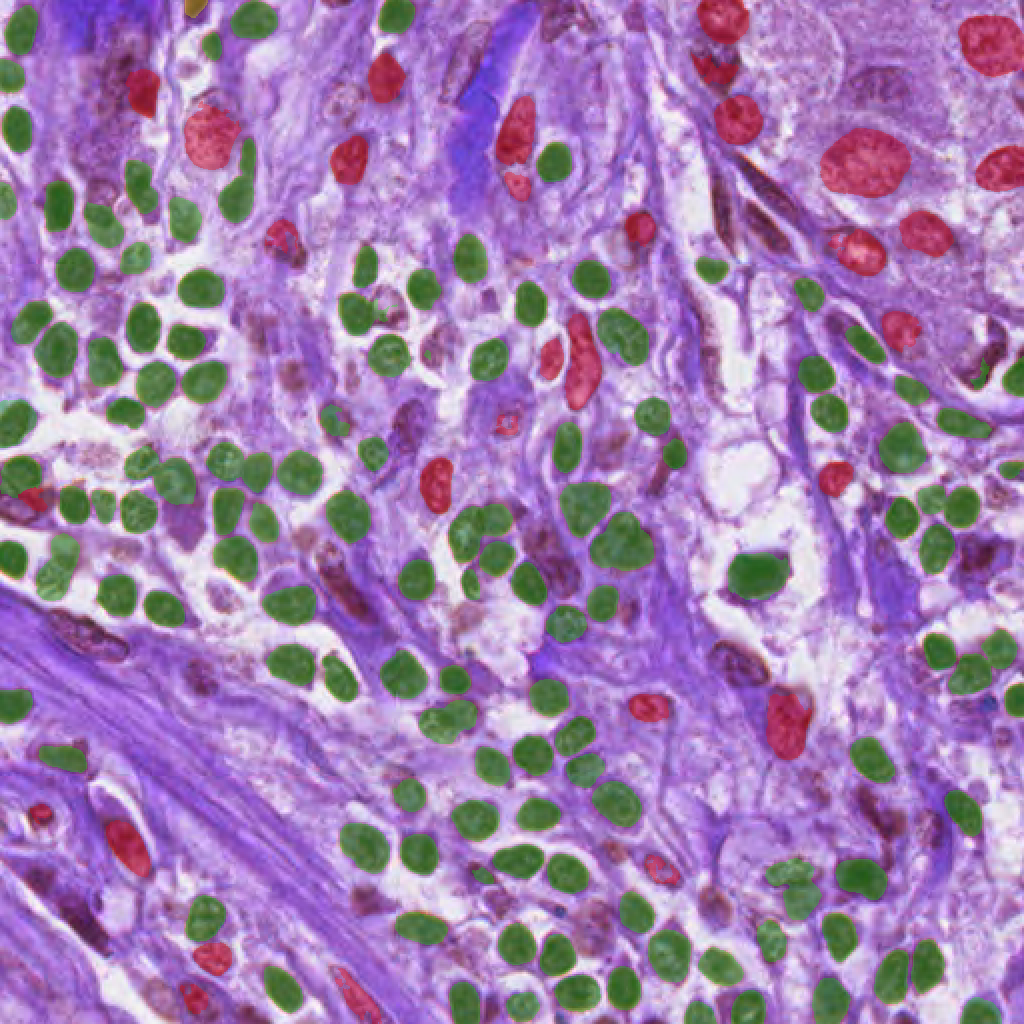
\includegraphics[width=\textwidth]{imgs/qual/monusac/hov1.png}
    \caption{Hovernet}
    \label{fig:monusac-hov1}
  \end{subfigure}
  \\
  \begin{subfigure}[b]{0.45\textwidth}
    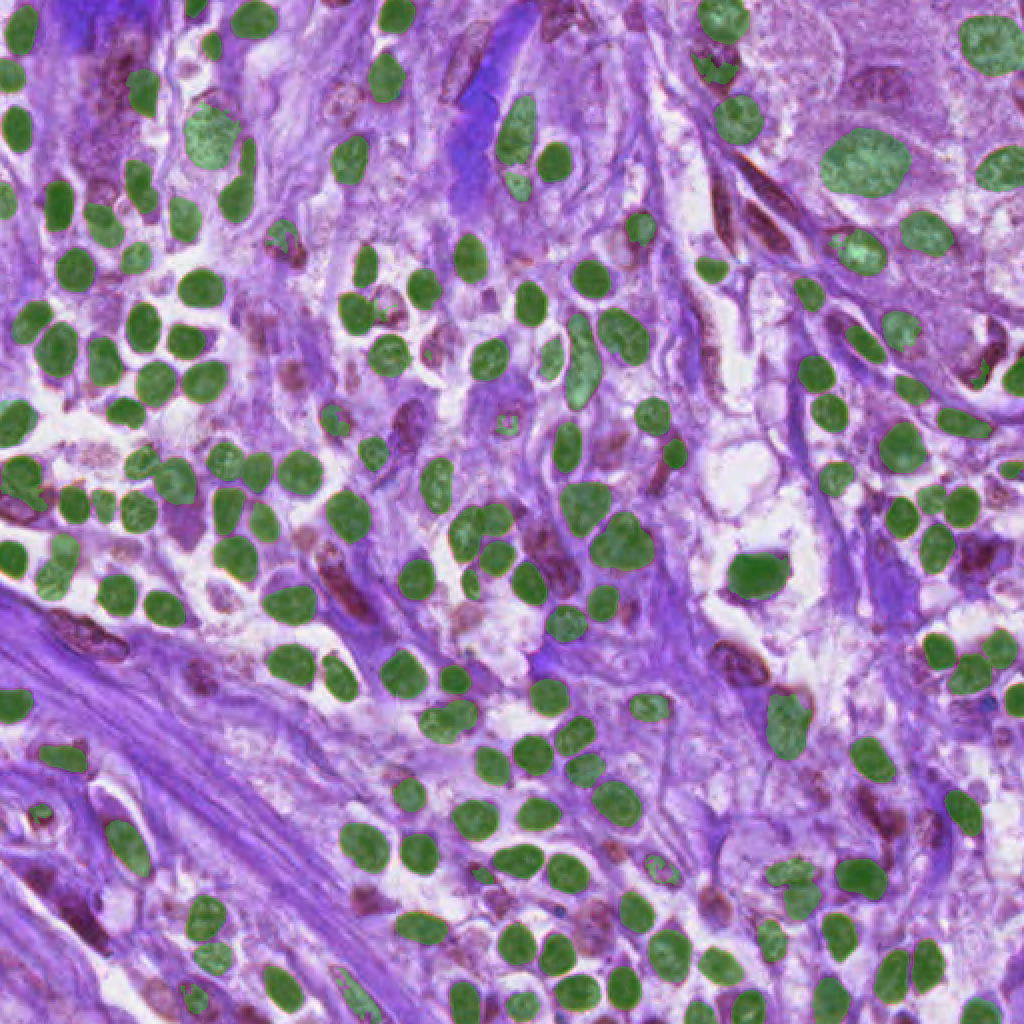
\includegraphics[width=\textwidth]{imgs/qual/monusac/gcn-full1.png}
    \caption{GCN}
    \label{fig:monusac-gcn1}
  \end{subfigure}
  \hfill
  \begin{subfigure}[b]{0.45\textwidth}
    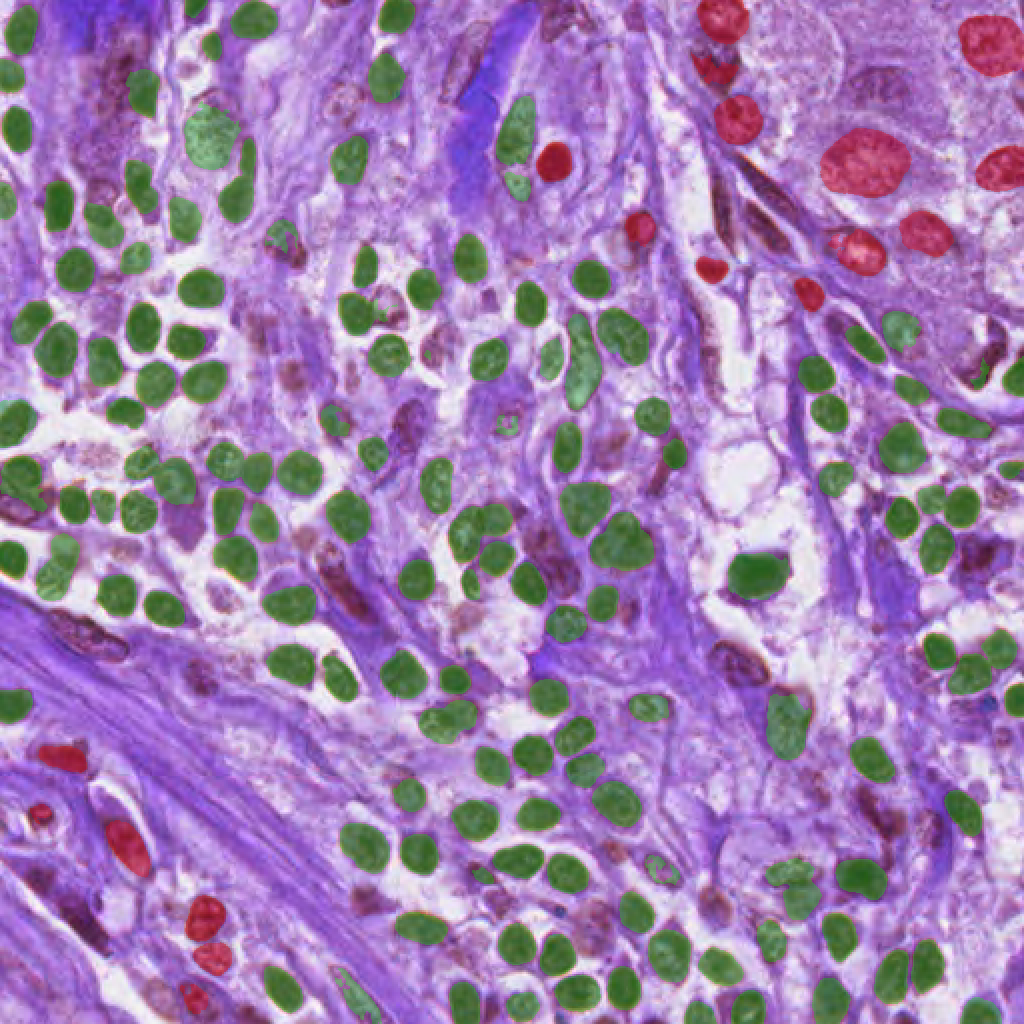
\includegraphics[width=\textwidth]{imgs/qual/monusac/no-morph1.png}
    \caption{Probabilities only}
    \label{fig:monusac-no-morph1}
  \end{subfigure}
  \\
  \begin{subfigure}[b]{0.45\textwidth}
    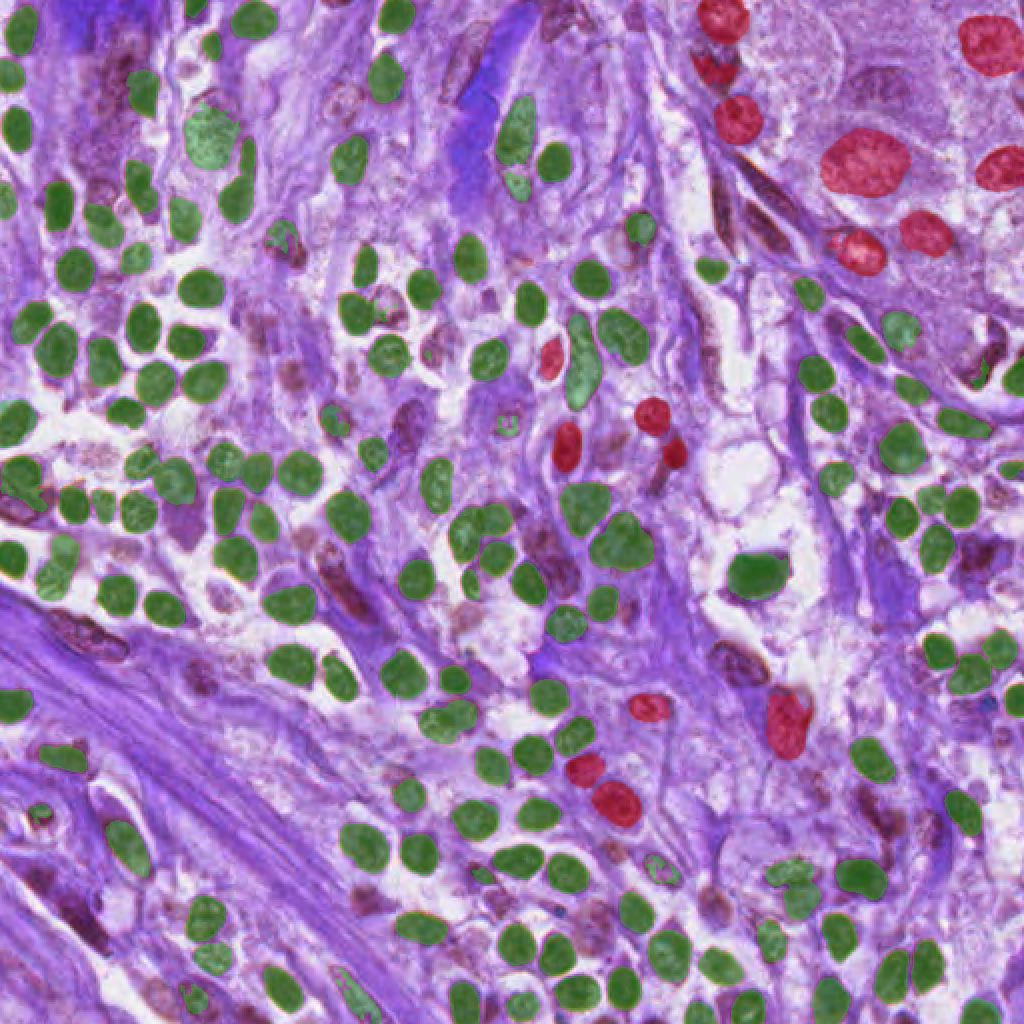
\includegraphics[width=\textwidth]{imgs/qual/monusac/no-prior1.png}
    \caption{Morphological features only}
    \label{fig:monusac-no-prior1}
  \end{subfigure}
  \hfill
  \begin{subfigure}[b]{0.45\textwidth}
    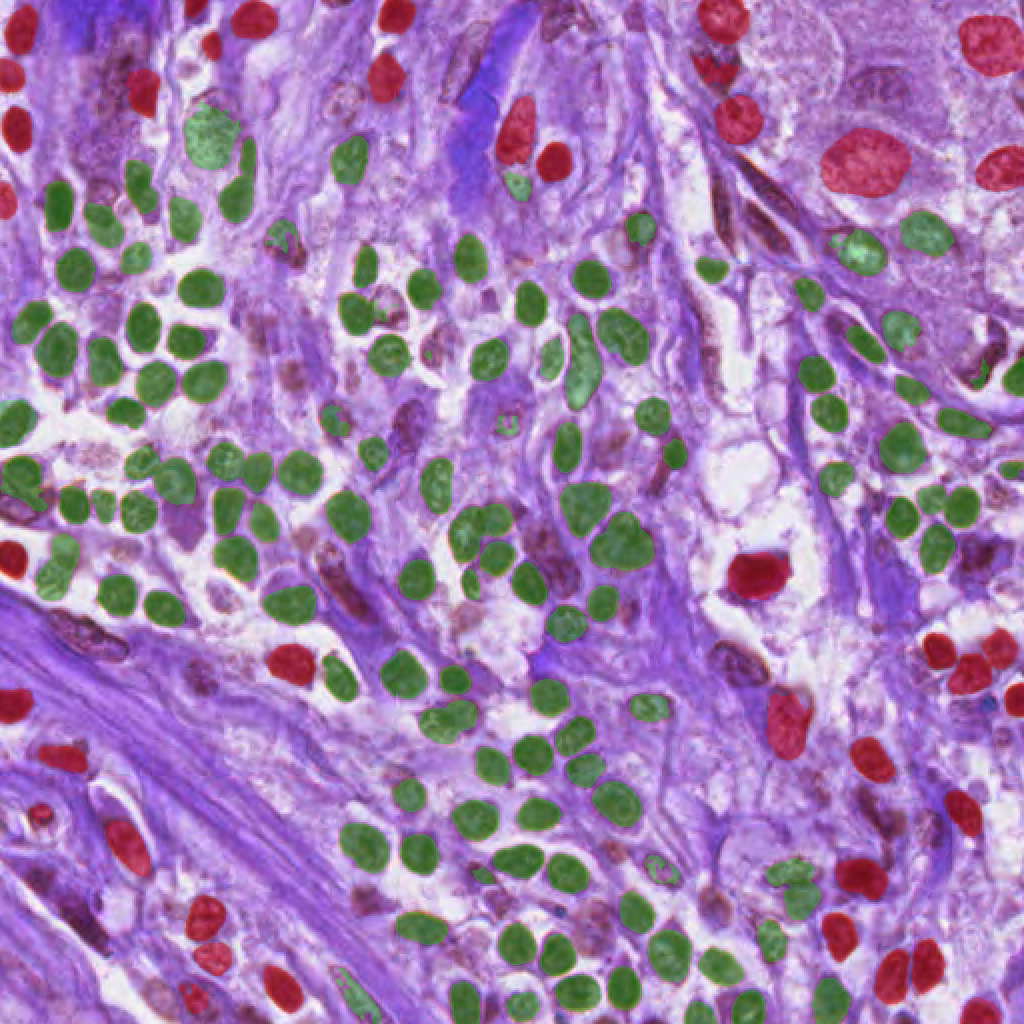
\includegraphics[width=\textwidth]{imgs/qual/monusac/void1.png}
    \caption{Void}
    \label{fig:monusac-void1}
  \end{subfigure}
  \caption{Illustration of the behaviour of the different models.}
  \label{fig:monusac-qual1}
\end{figure}

\begin{figure}[H]
  \centering
  \begin{subfigure}[b]{0.45\textwidth}
    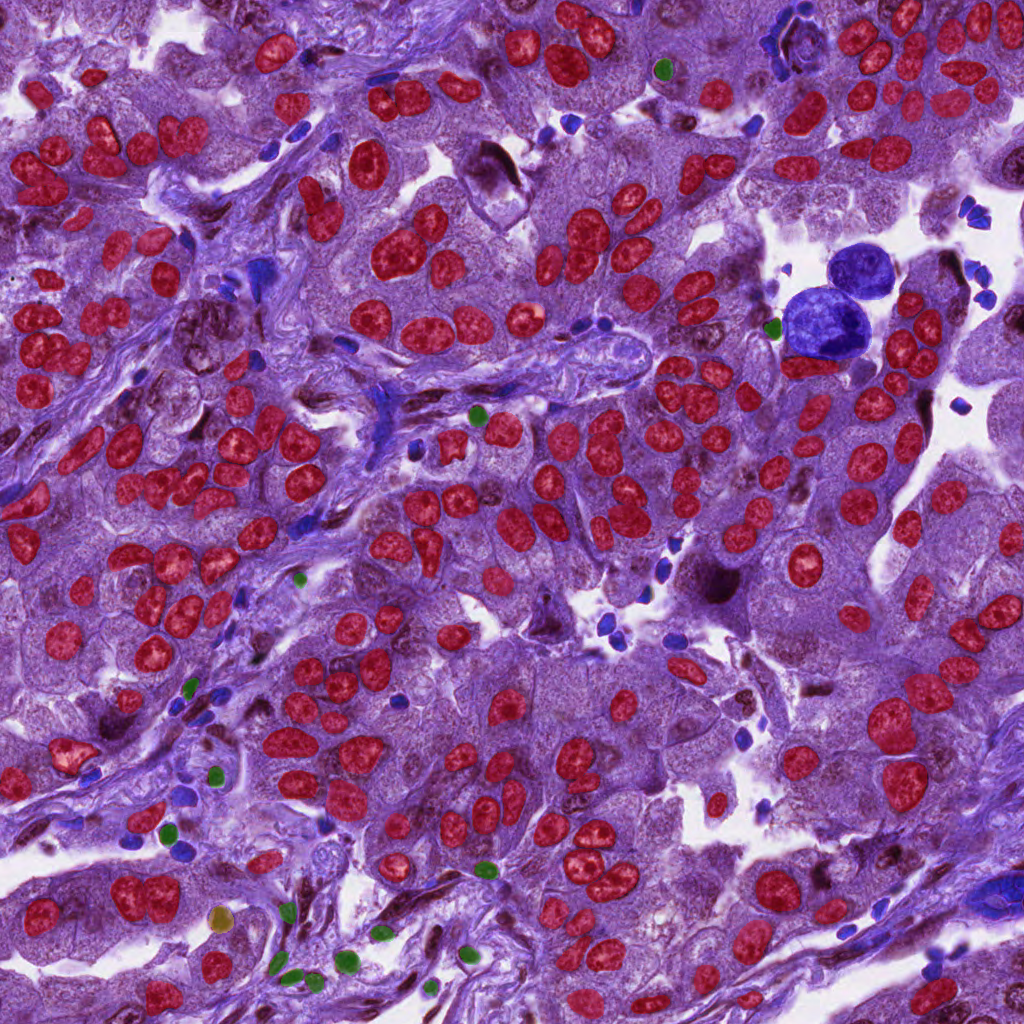
\includegraphics[width=\textwidth]{imgs/qual/monusac/gt3.overlay.png}
    \caption{GT}
    \label{fig:monusac-gt3}
  \end{subfigure}
  \hfill
  \begin{subfigure}[b]{0.45\textwidth}
    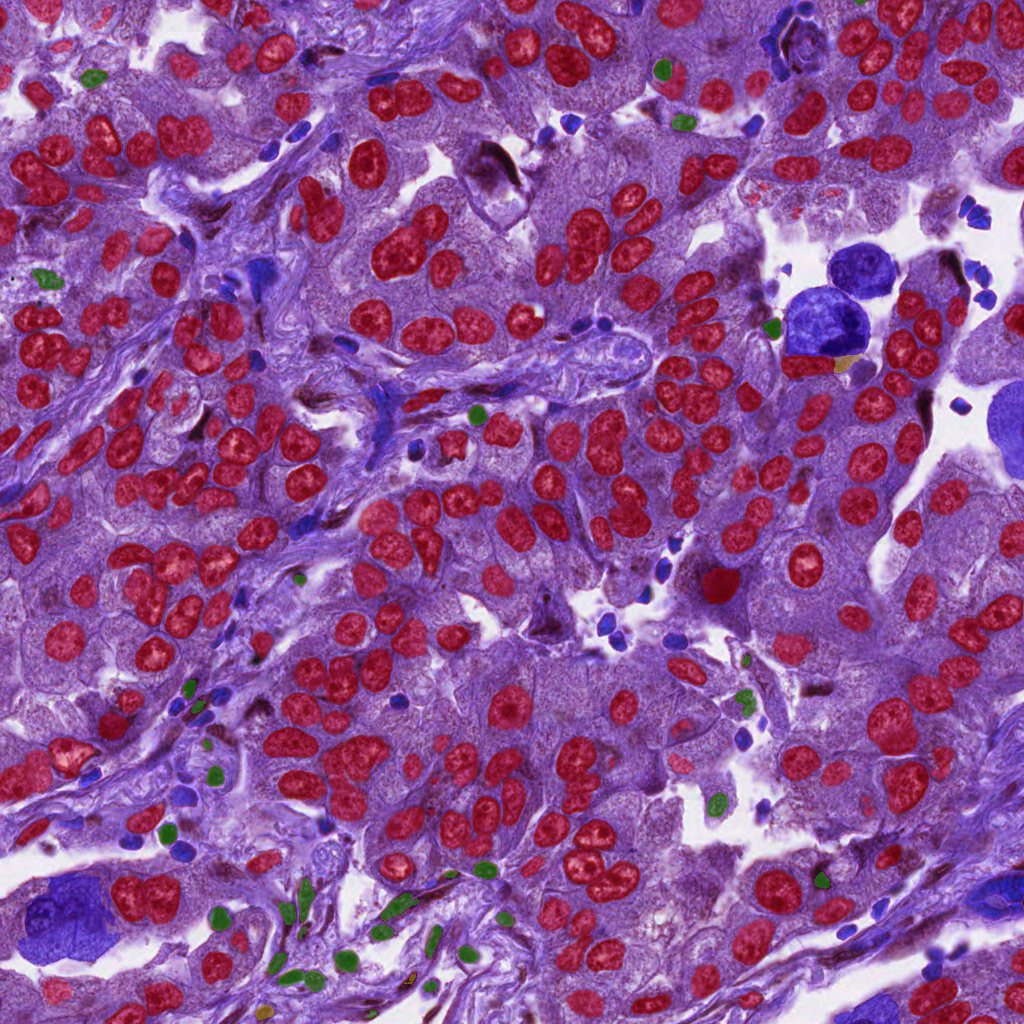
\includegraphics[width=\textwidth]{imgs/qual/monusac/hov3.png}
    \caption{Hovernet}
    \label{fig:monusac-hov3}
  \end{subfigure}
  \\
  \begin{subfigure}[b]{0.45\textwidth}
    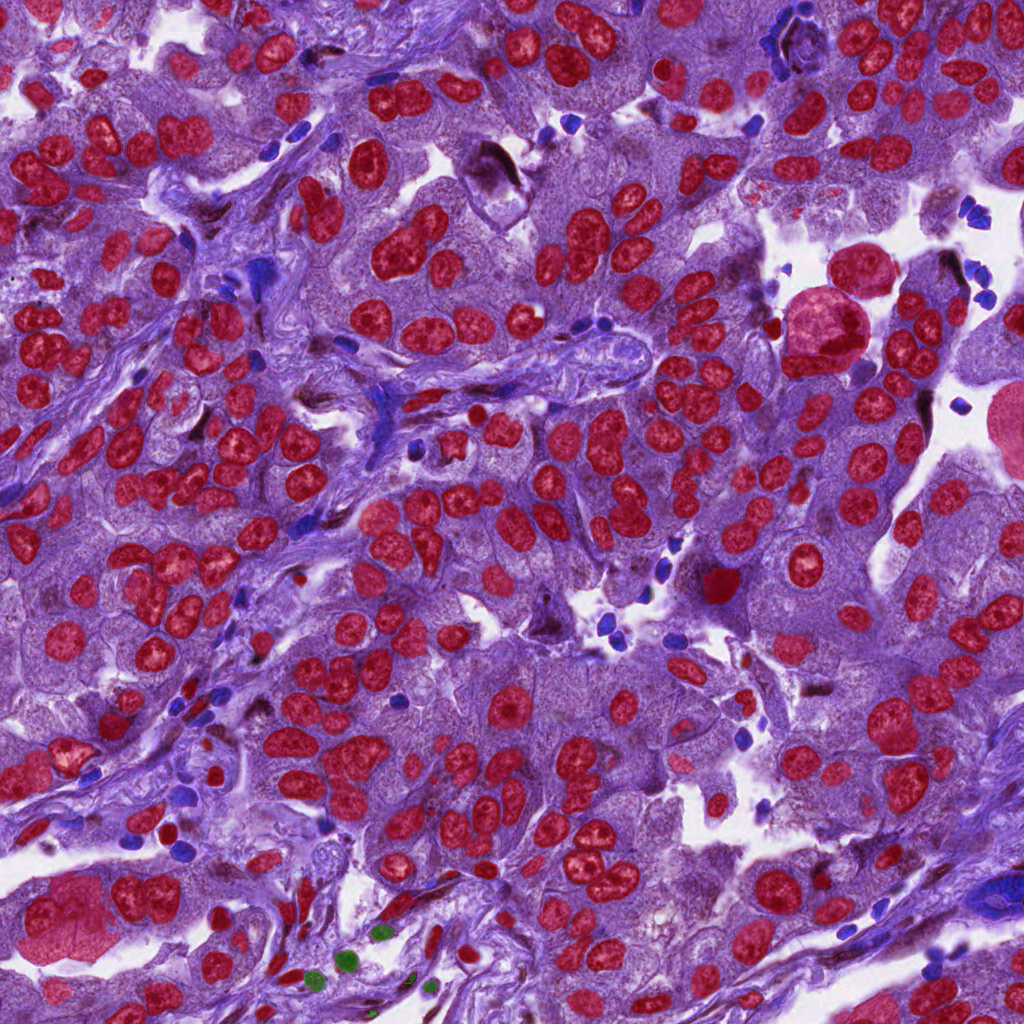
\includegraphics[width=\textwidth]{imgs/qual/monusac/gcn-full3.png}
    \caption{GCN}
    \label{fig:monusac-gcn3}
  \end{subfigure}
  \hfill
  \begin{subfigure}[b]{0.45\textwidth}
    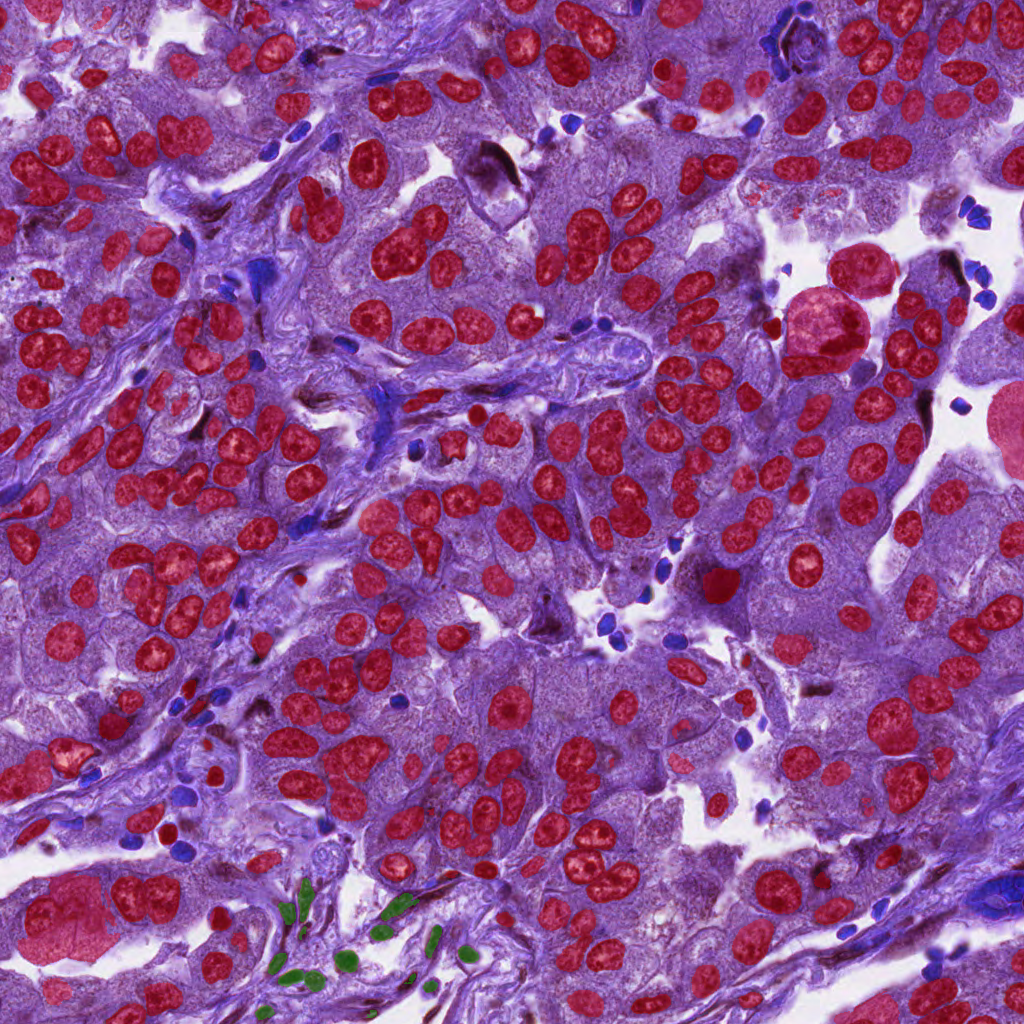
\includegraphics[width=\textwidth]{imgs/qual/monusac/no-morph3.png}
    \caption{Probabilities only}
    \label{fig:monusac-no-morph3}
  \end{subfigure}
  \\
  \begin{subfigure}[b]{0.45\textwidth}
    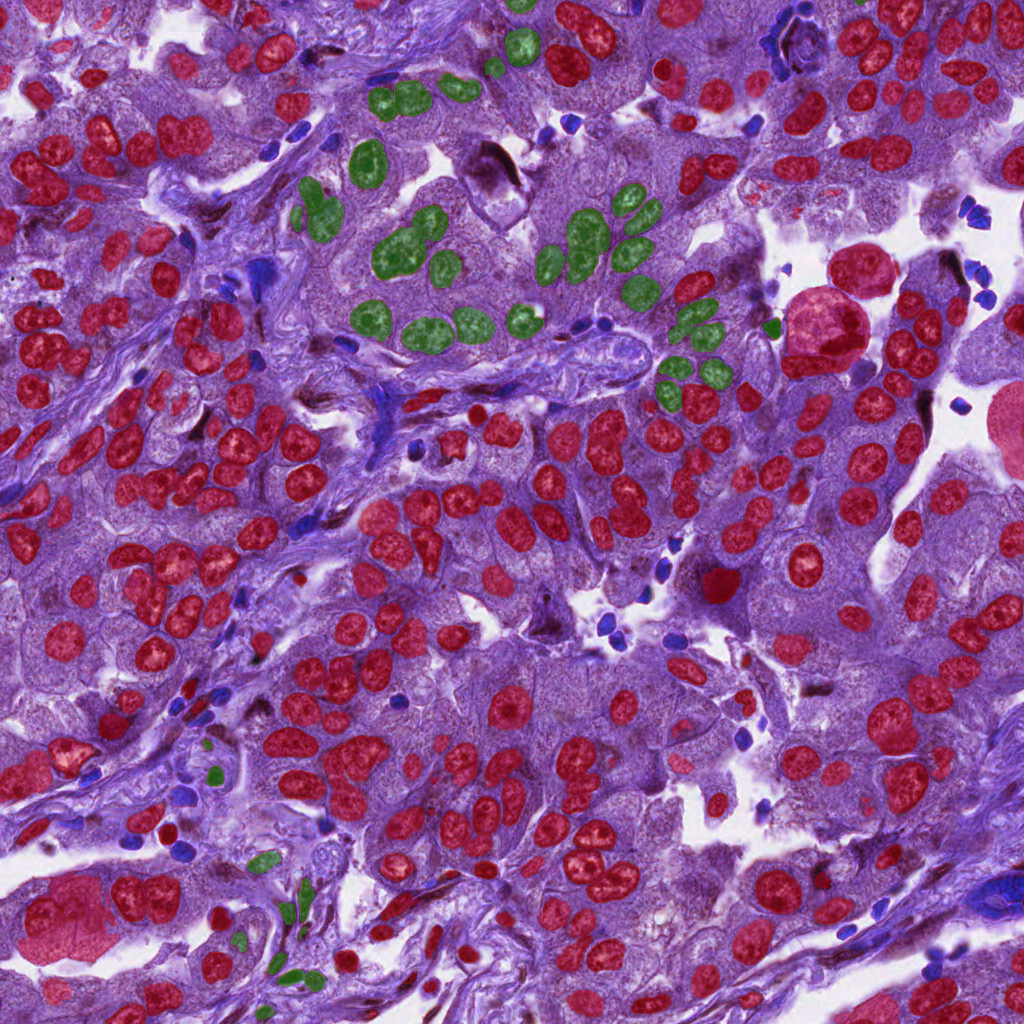
\includegraphics[width=\textwidth]{imgs/qual/monusac/no-prior3.png}
    \caption{Morphological features only}
    \label{fig:monusac-no-prior3}
  \end{subfigure}
  \hfill
  \begin{subfigure}[b]{0.45\textwidth}
    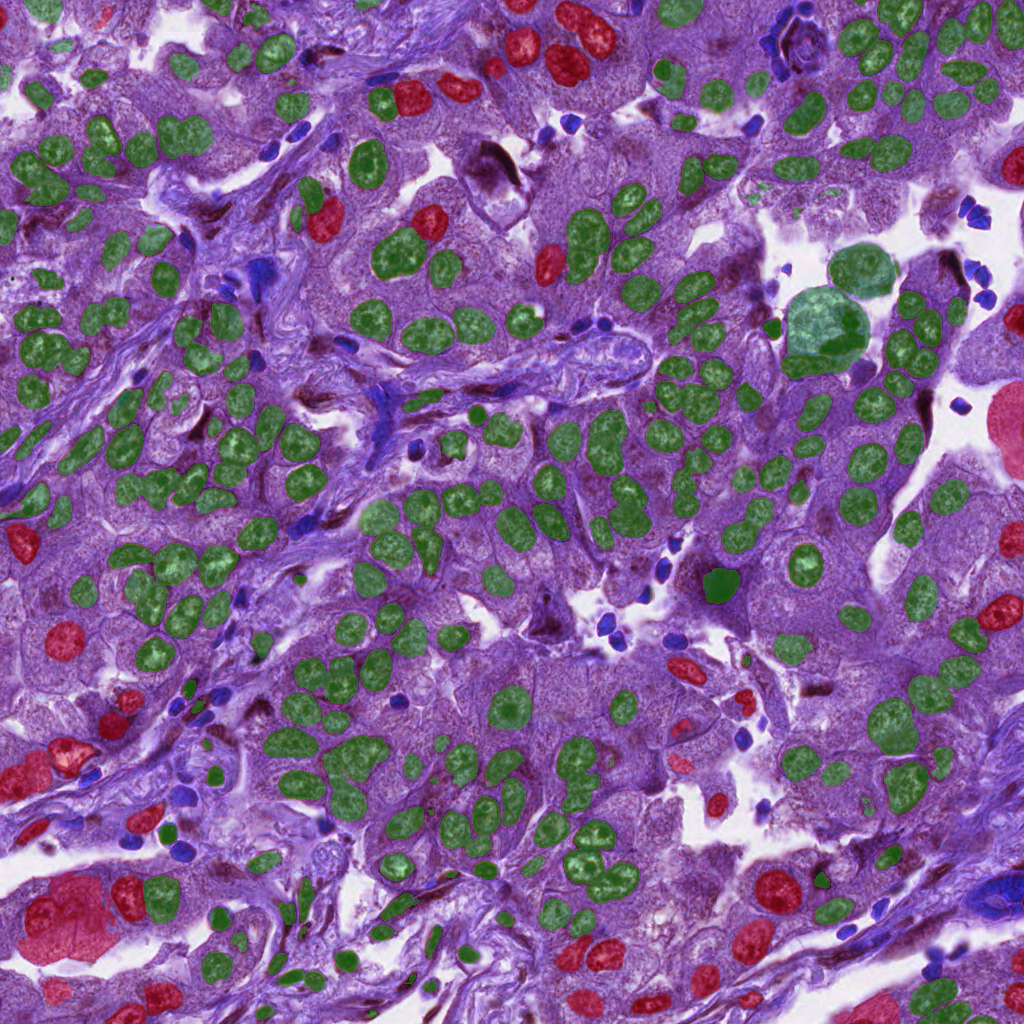
\includegraphics[width=\textwidth]{imgs/qual/monusac/void3.png}
    \caption{Void}
    \label{fig:monusac-void3}
  \end{subfigure}
  \caption{Another illustration of the behaviour of the different models.}
  \label{fig:monusac-qual3}
\end{figure}


\subsection{DigiPatics breast}

Let's start the qualitative analysis of this section with a question. Given the following three images with their ground truth on top. Which of them would you think is going to give less trouble to the graph neural networks? If you have read the previous two sections the answer should be obvious by now.

\begin{figure}[H]
    \centering
    \begin{subfigure}[b]{0.3\textwidth}
    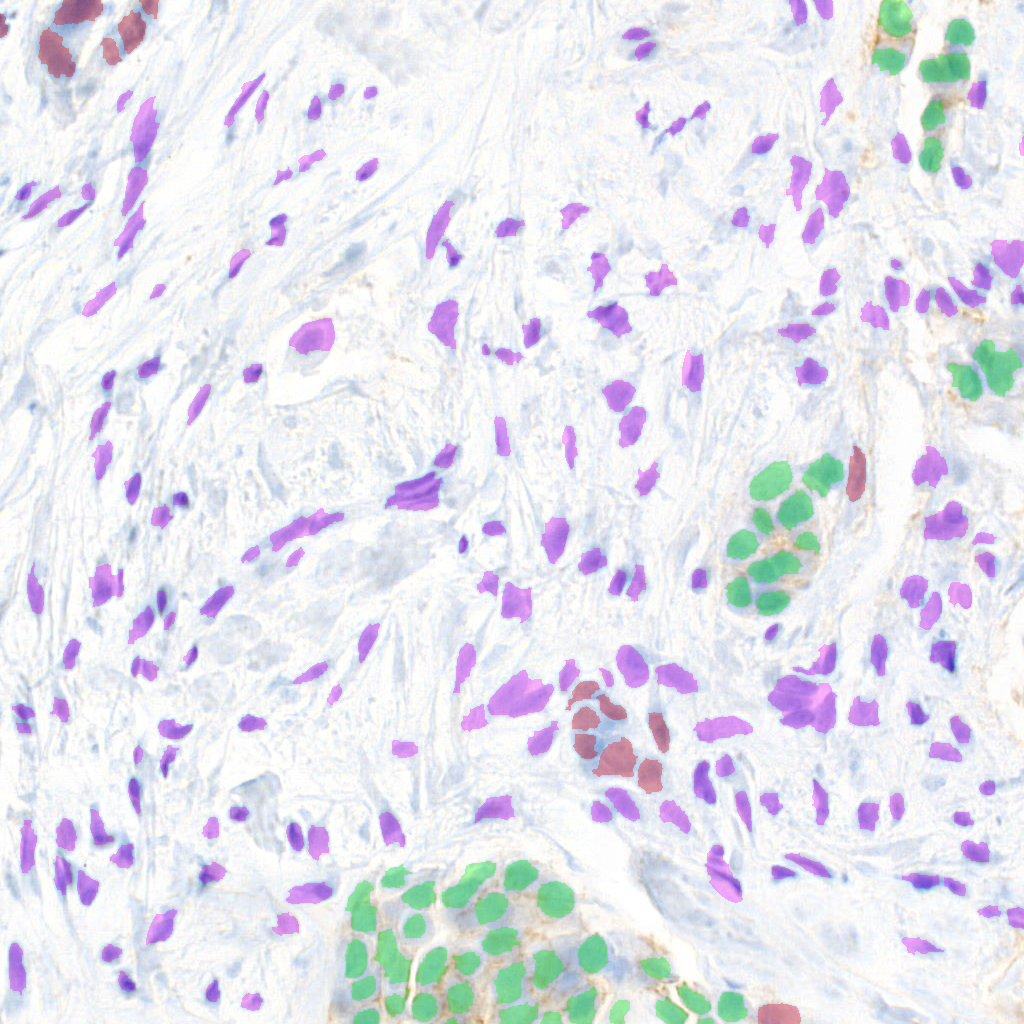
\includegraphics[width=\textwidth]{imgs/qual/breast/gt1.overlay.png}
    \label{fig:breast-gt1}
  \end{subfigure}
  \begin{subfigure}[b]{0.3\textwidth}
    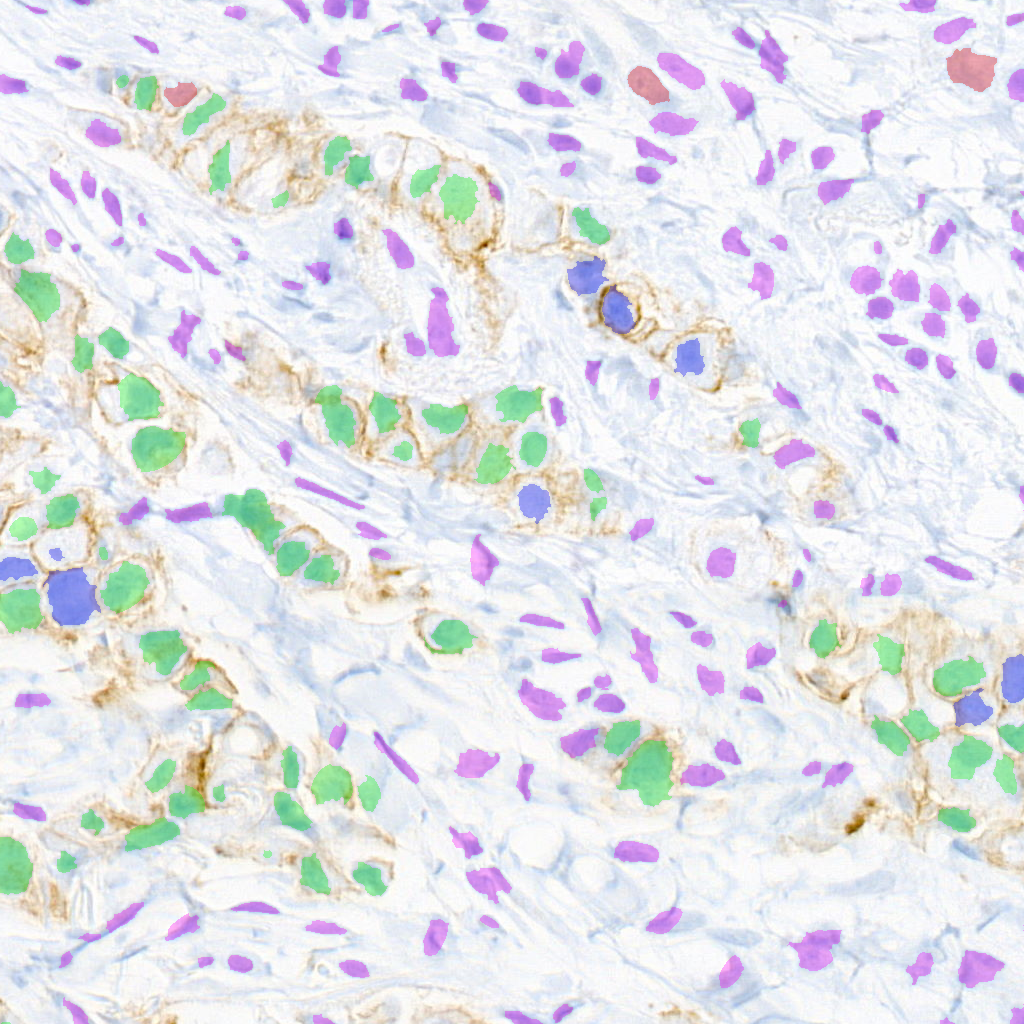
\includegraphics[width=\textwidth]{imgs/qual/breast/gt2.overlay.png}
    \label{fig:breast-gt2}
  \end{subfigure}
  \begin{subfigure}[b]{0.3\textwidth}
    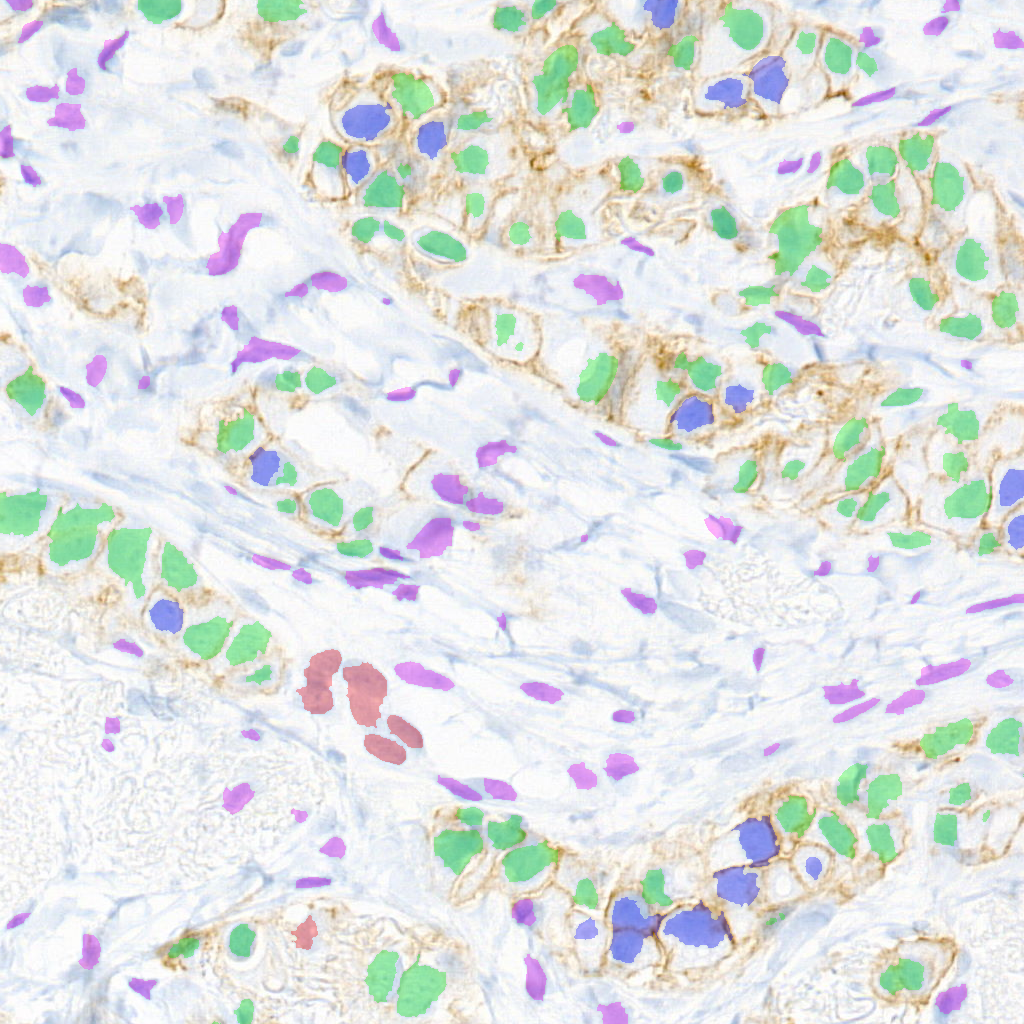
\includegraphics[width=\textwidth]{imgs/qual/breast/gt3.overlay.png}
    \label{fig:breast-gt3}
  \end{subfigure}
    \caption{Three examples with their ground truth overlayed on top.}
    \label{fig:breast-ex}
\end{figure}

That's right, the left one. It has clearly identifiable groups. The other two also have nests of cells but in between there are cells of other classes. In the first image the nests are clearly defined and separated between each others. Now comes the second question. Watch the next image in \autoref{fig:breast-hov1}, which is the output of Hovernet, and try to predict which are going to be the groups detected by the GCN trained with all the features, with probabilities only, with morphological features only and with features at all.

\begin{figure}[H]
    \centering
    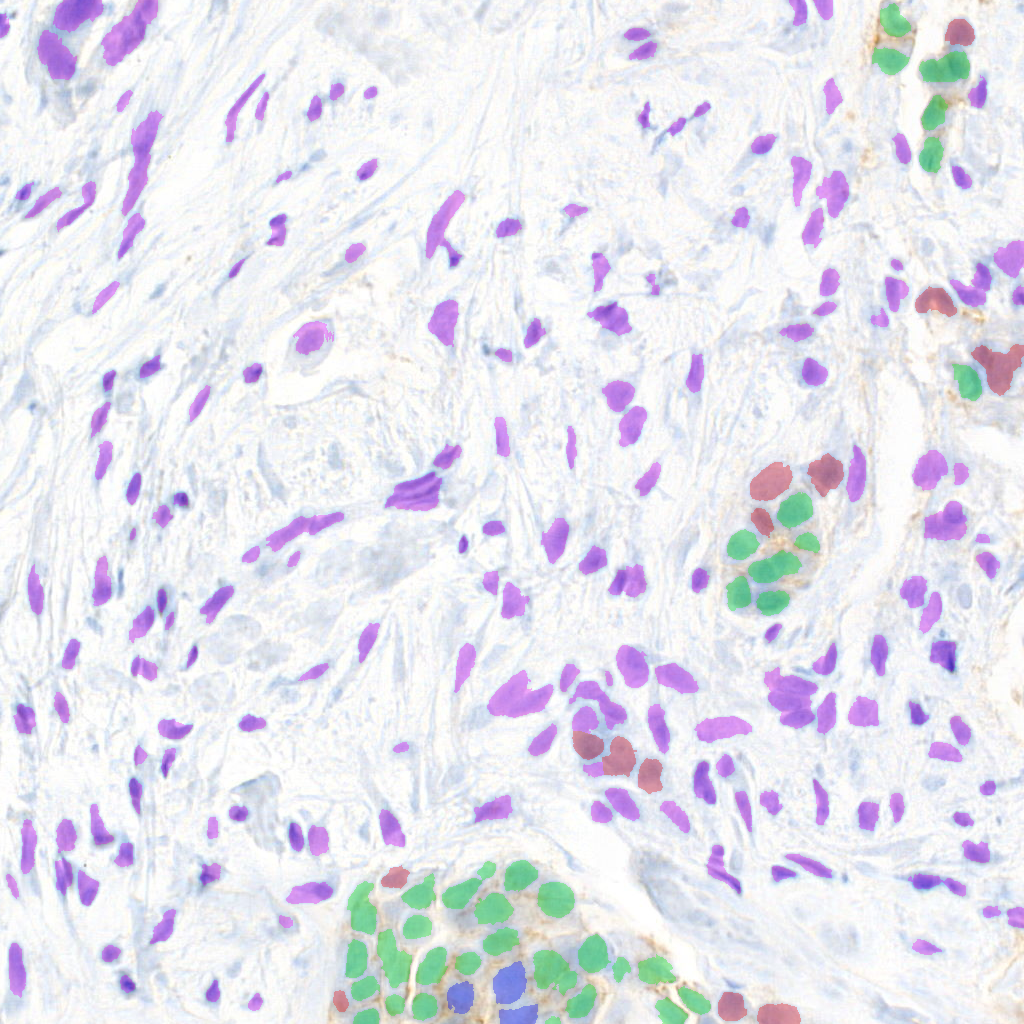
\includegraphics[width=0.5\textwidth]{imgs/qual/breast/hov1.png}
    \caption{Output of Hovernet for the leftmost image of \autoref{fig:breast-ex}.}
    \label{fig:breast-hov1}
\end{figure}

This question was more tricky. Although GNNs behave predictably, there is still margin for uncertainty. The GCN with all the features has made the green cells eat their neighbours although it missed the group at top right which is detected by the model trained only with probabilities. On the other hand, the model that does not have Hovernet probabilities has predicted some red cells where the other predicted red or magenta. And the void model has played the safest of them all by just classifying everything with the dominant class. Note that being safe does not mean being good. It is just a poetic license to state that it did not bother trying to identify minority groups.

\begin{figure}[H]
  \centering
  \begin{subfigure}[b]{0.45\textwidth}
    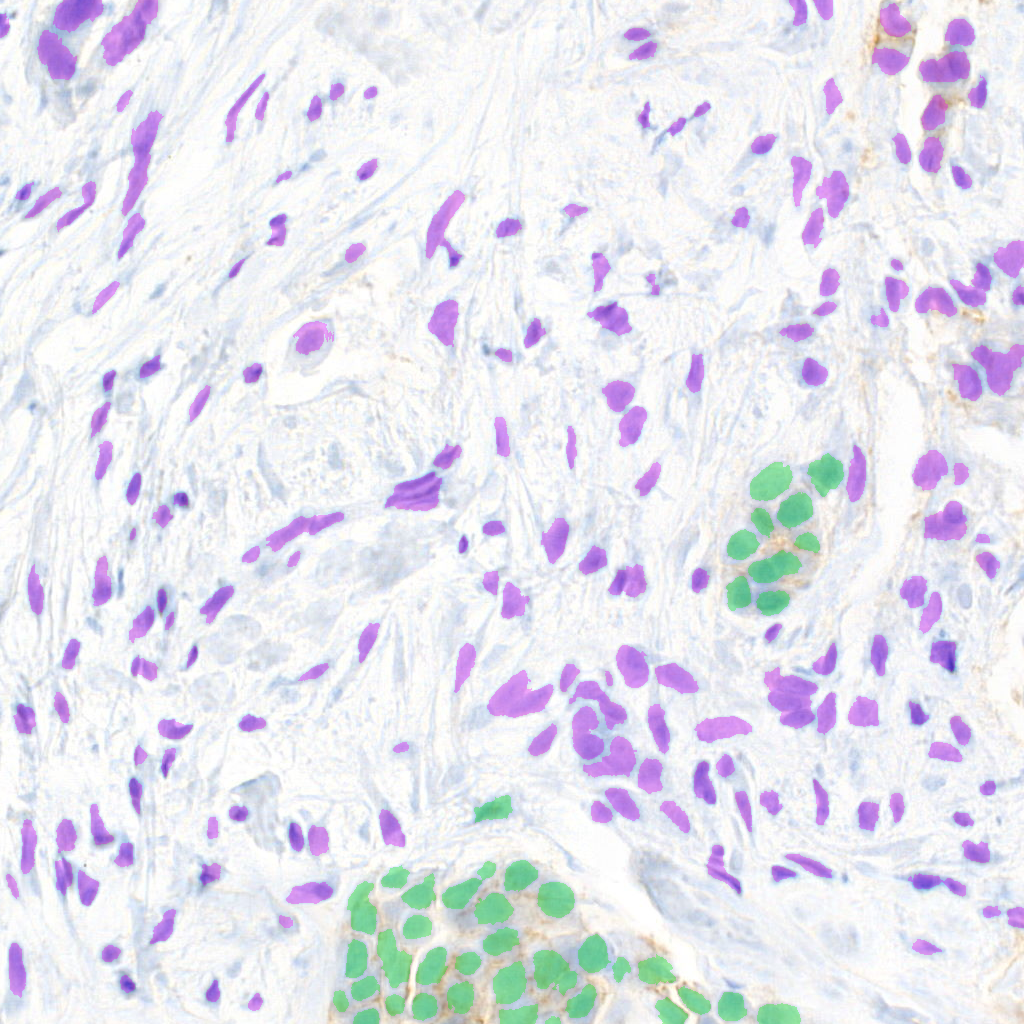
\includegraphics[width=\textwidth]{imgs/qual/breast/gcn-full1.png}
    \caption{GCN}
    \label{fig:breast-gt1}
  \end{subfigure}
  \hfill
  \begin{subfigure}[b]{0.45\textwidth}
    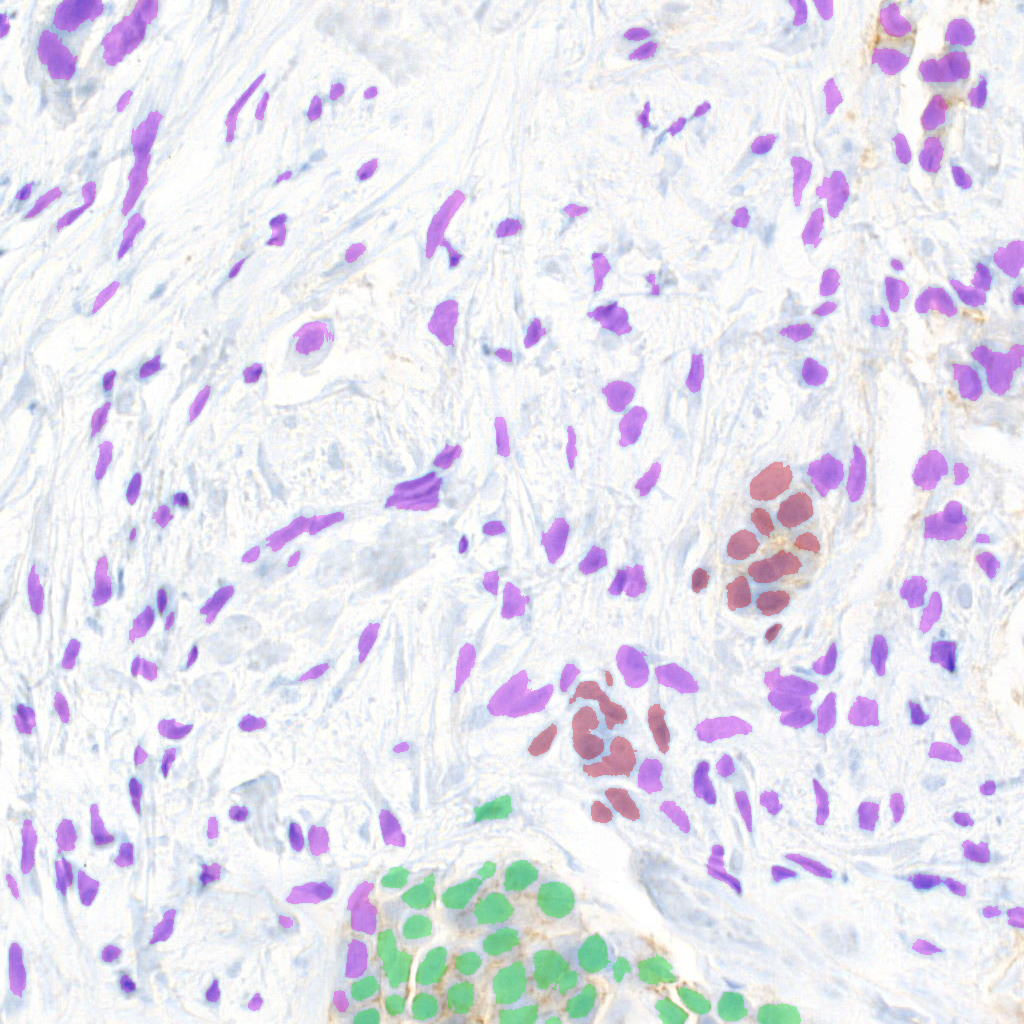
\includegraphics[width=\textwidth]{imgs/qual/breast/no-prior1.png}
    \caption{Morphological features}
    \label{fig:breast-no-prior1}
  \end{subfigure}
  \\
  \begin{subfigure}[b]{0.45\textwidth}
    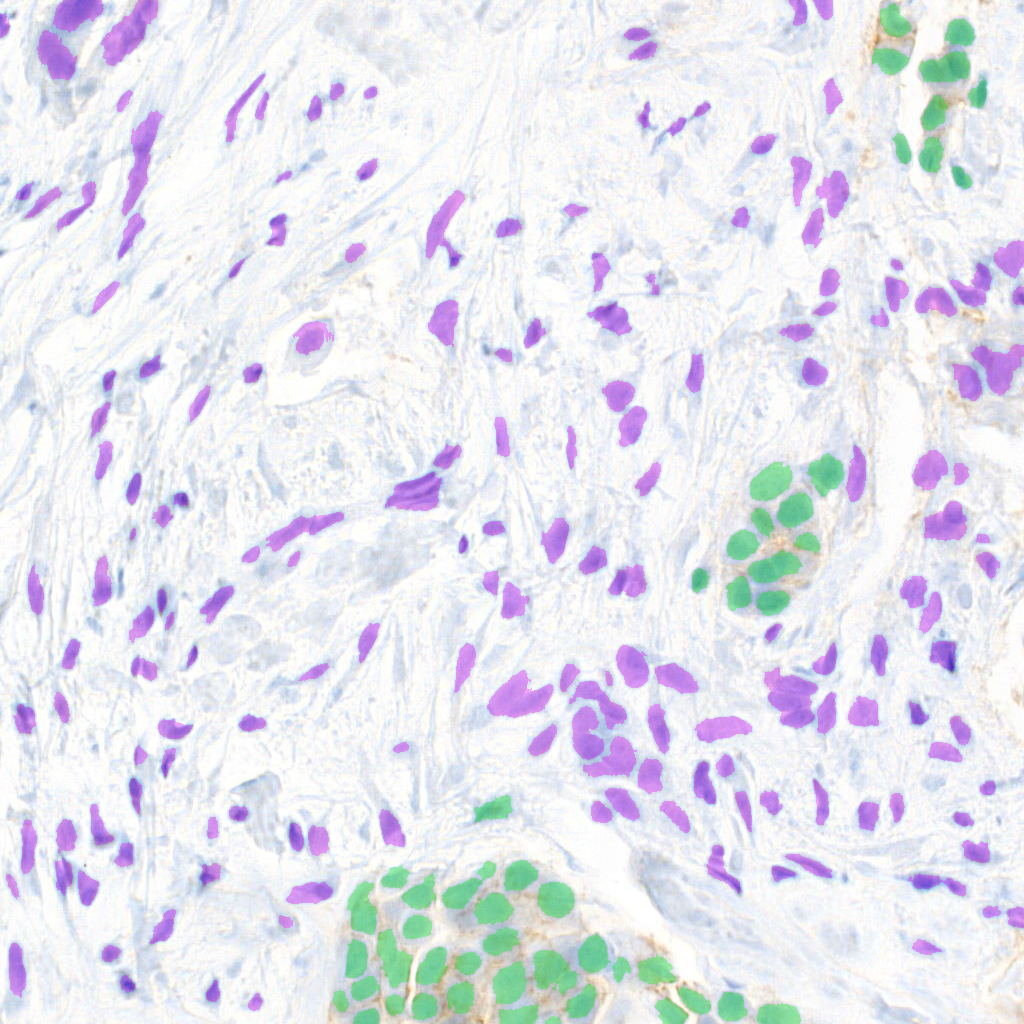
\includegraphics[width=\textwidth]{imgs/qual/breast/no-morph1.png}
    \caption{Probabilities}
    \label{fig:breast-no-morph1}
  \end{subfigure}
  \hfill
  \begin{subfigure}[b]{0.45\textwidth}
    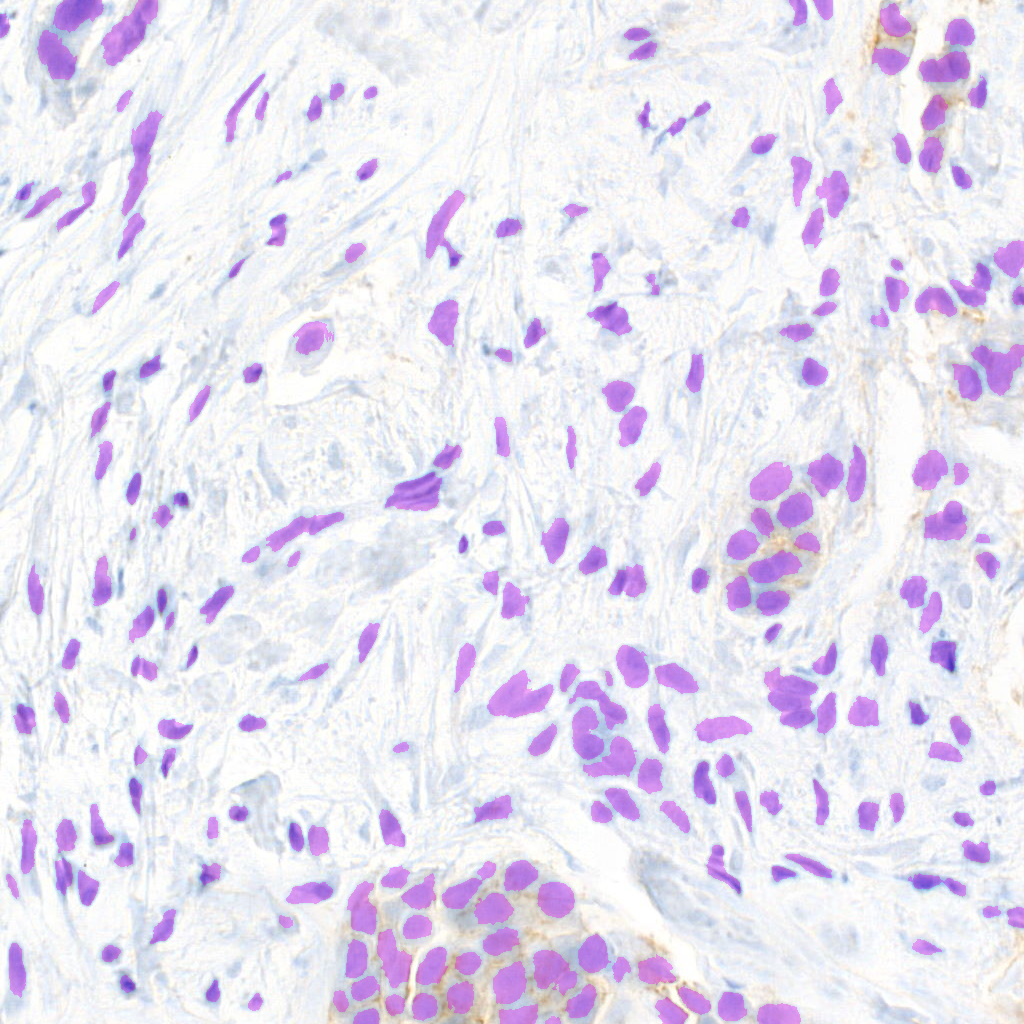
\includegraphics[width=\textwidth]{imgs/qual/breast/void1.png}
    \caption{Void}
    \label{fig:consep-void}
  \end{subfigure}
  \caption{Output of the GCN trained with different sets of input features.}
  \label{fig:breast-qual1}
\end{figure}

In \autoref{fig:breast-qual2} and \autoref{fig:breast-qual3} there are the outputs for the other two images from the beginning. Graph networks try to find clusters, sometimes they guess it right, sometimes they don't. Hovernet, as usual, tries to identify lonely cells correctly. Again, sometimes it works, sometimes it does not.


\begin{figure}[H]
  \centering
  \begin{subfigure}[b]{0.45\textwidth}
    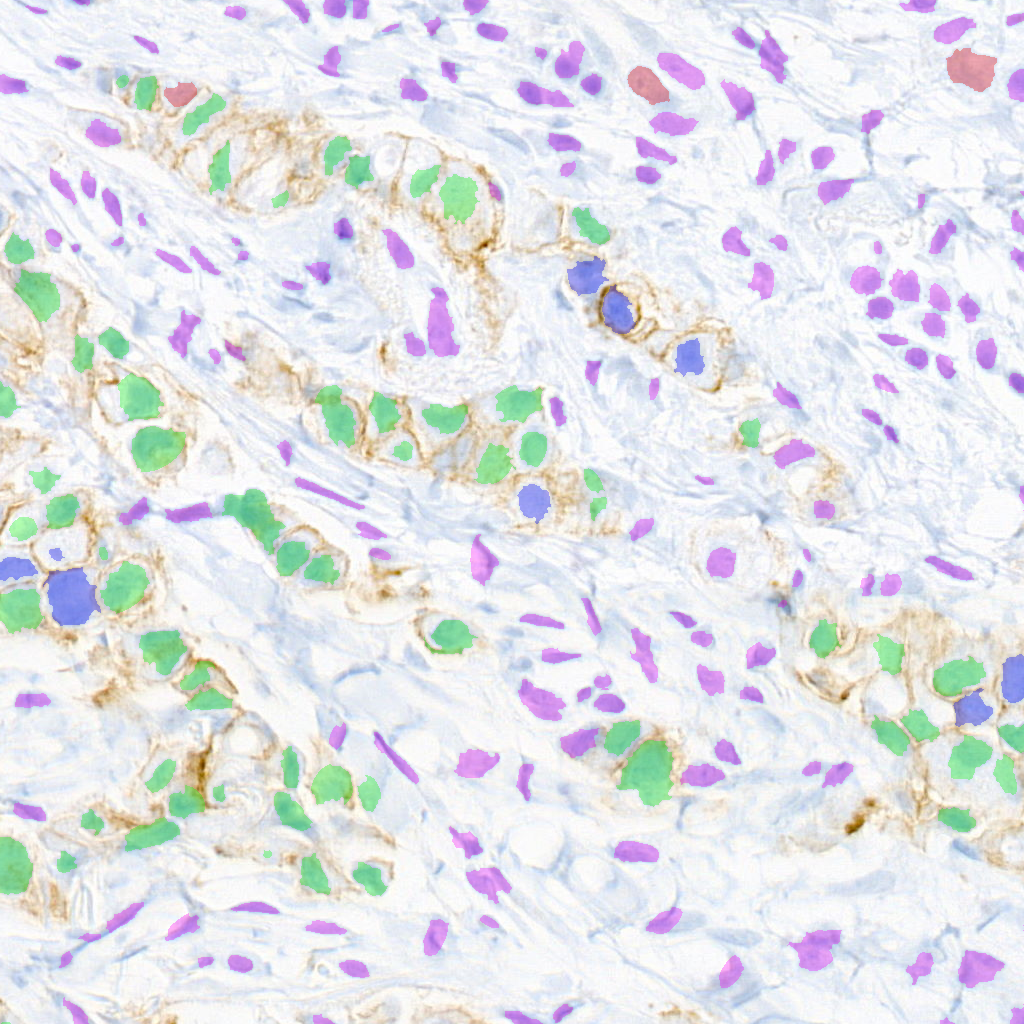
\includegraphics[width=\textwidth]{imgs/qual/breast/gt2.overlay.png}
    \caption{GT}
    \label{fig:breast-gt2}
  \end{subfigure}
  \hfill
  \begin{subfigure}[b]{0.45\textwidth}
    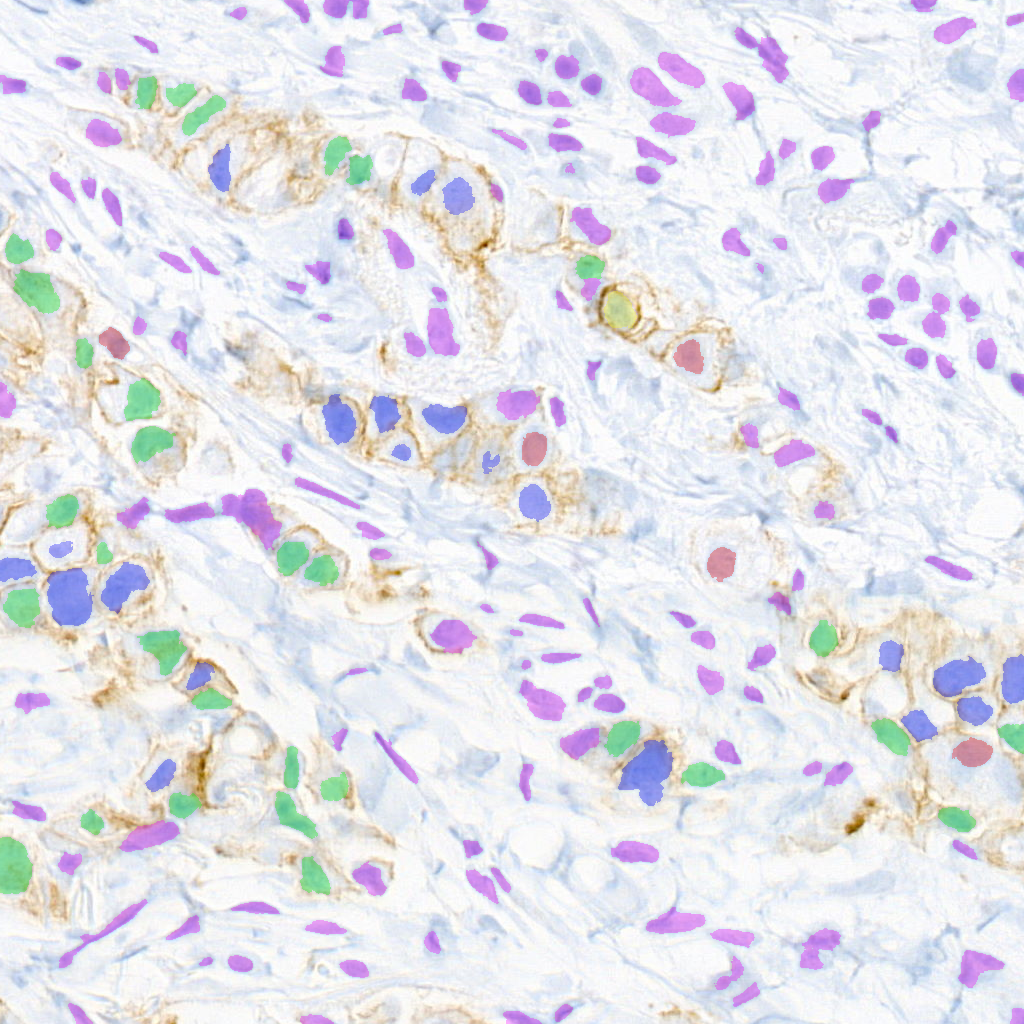
\includegraphics[width=\textwidth]{imgs/qual/breast/hov2.png}
    \caption{Hovernet}
    \label{fig:breast-hov2}
  \end{subfigure}
  \\
  \begin{subfigure}[b]{0.45\textwidth}
    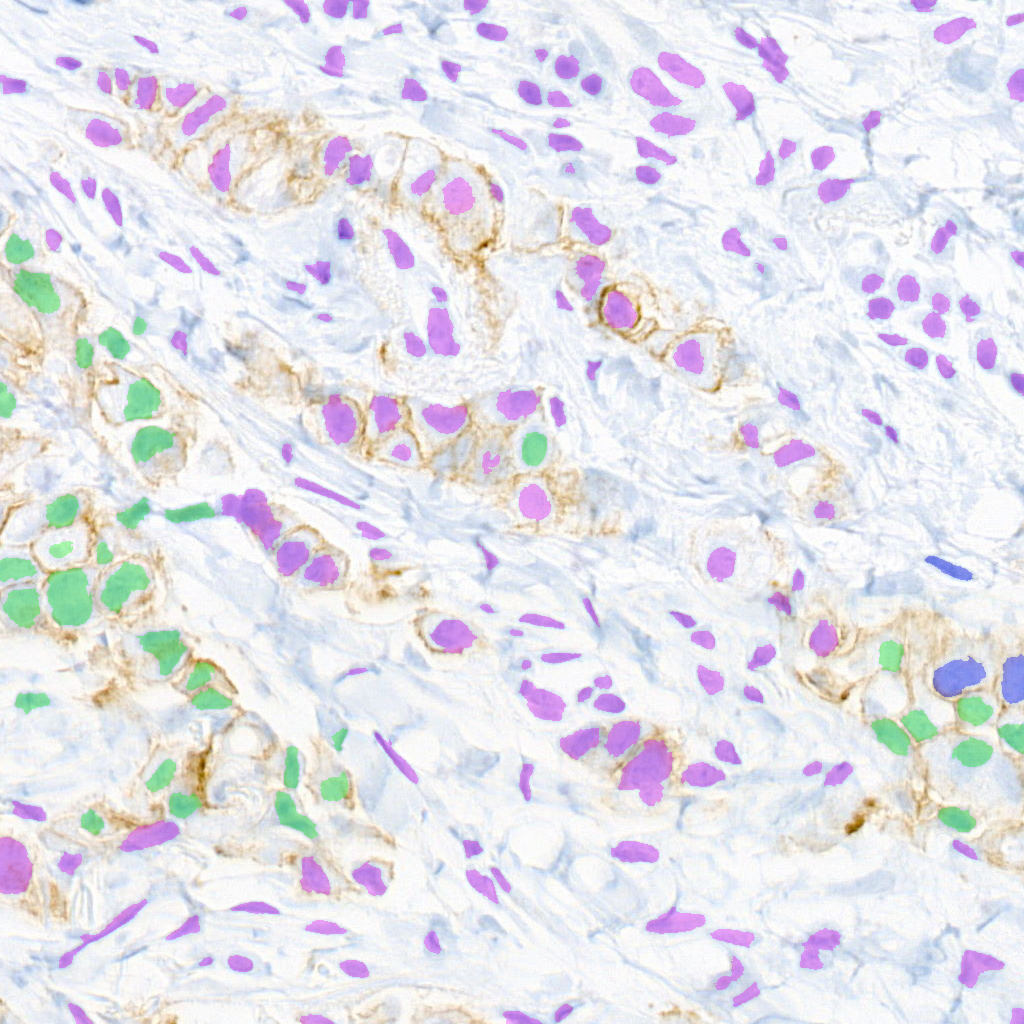
\includegraphics[width=\textwidth]{imgs/qual/breast/gcn-full2.png}
    \caption{GCN}
    \label{fig:breast-gcn2}
  \end{subfigure}
  \hfill
  \begin{subfigure}[b]{0.45\textwidth}
    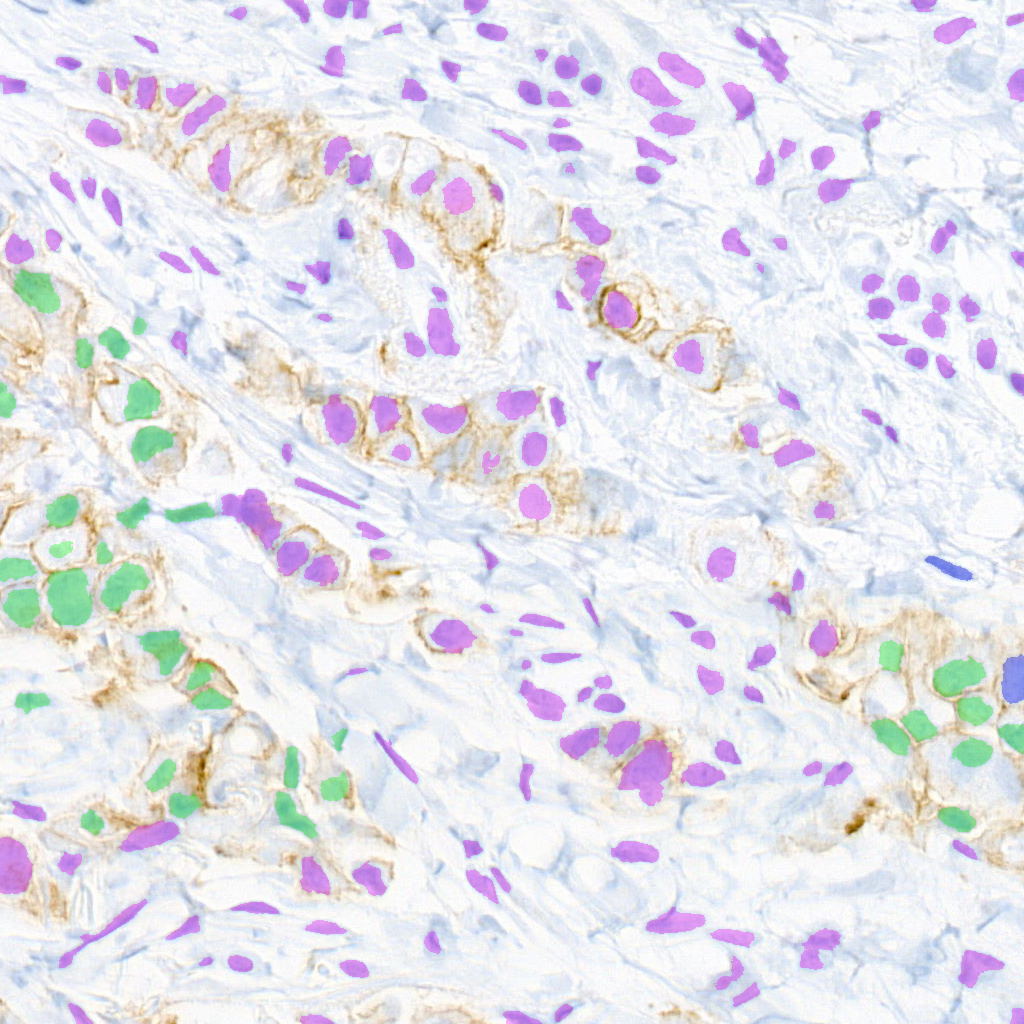
\includegraphics[width=\textwidth]{imgs/qual/breast/no-morph2.png}
    \caption{Probabilities only}
    \label{fig:breast-no-morph2}
  \end{subfigure}
  \\
  \begin{subfigure}[b]{0.45\textwidth}
    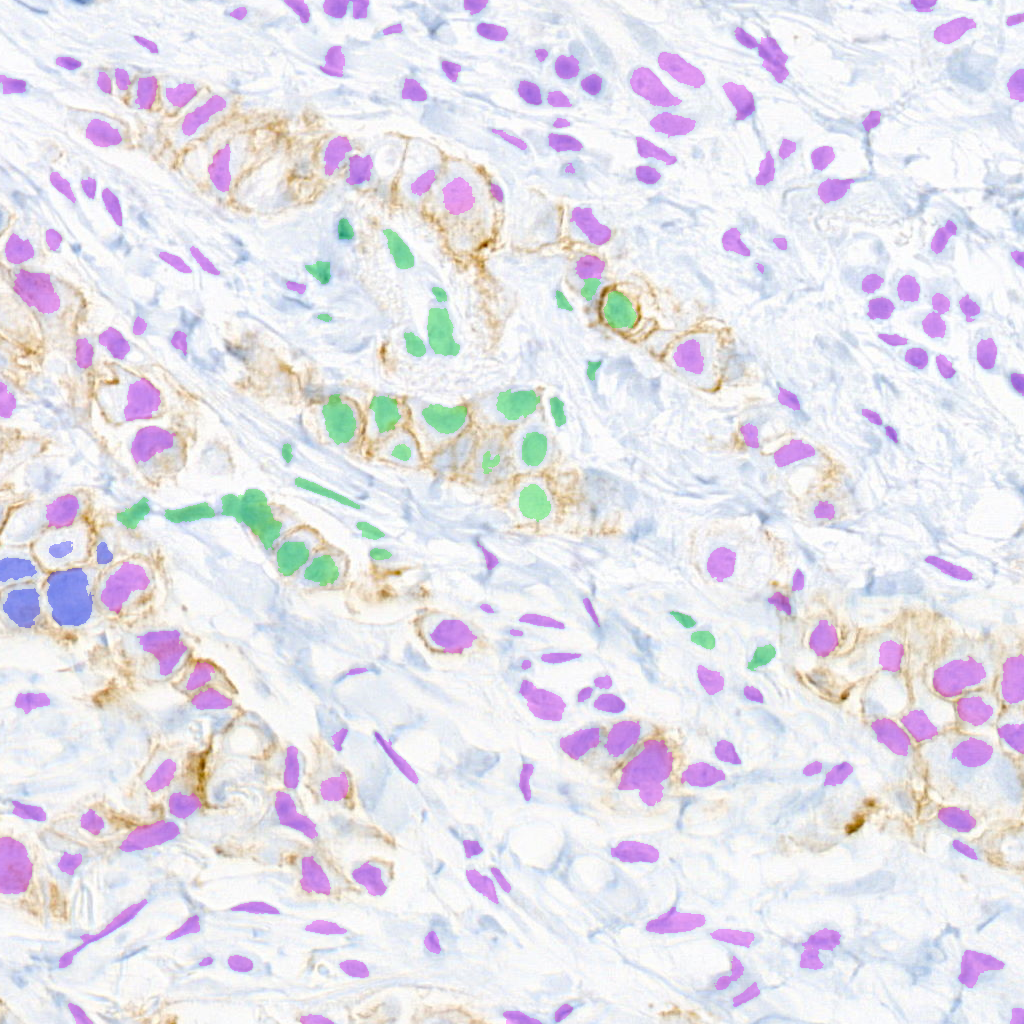
\includegraphics[width=\textwidth]{imgs/qual/breast/no-prior2.png}
    \caption{Morphological features only}
    \label{fig:breast-no-prior2}
  \end{subfigure}
  \hfill
  \begin{subfigure}[b]{0.45\textwidth}
    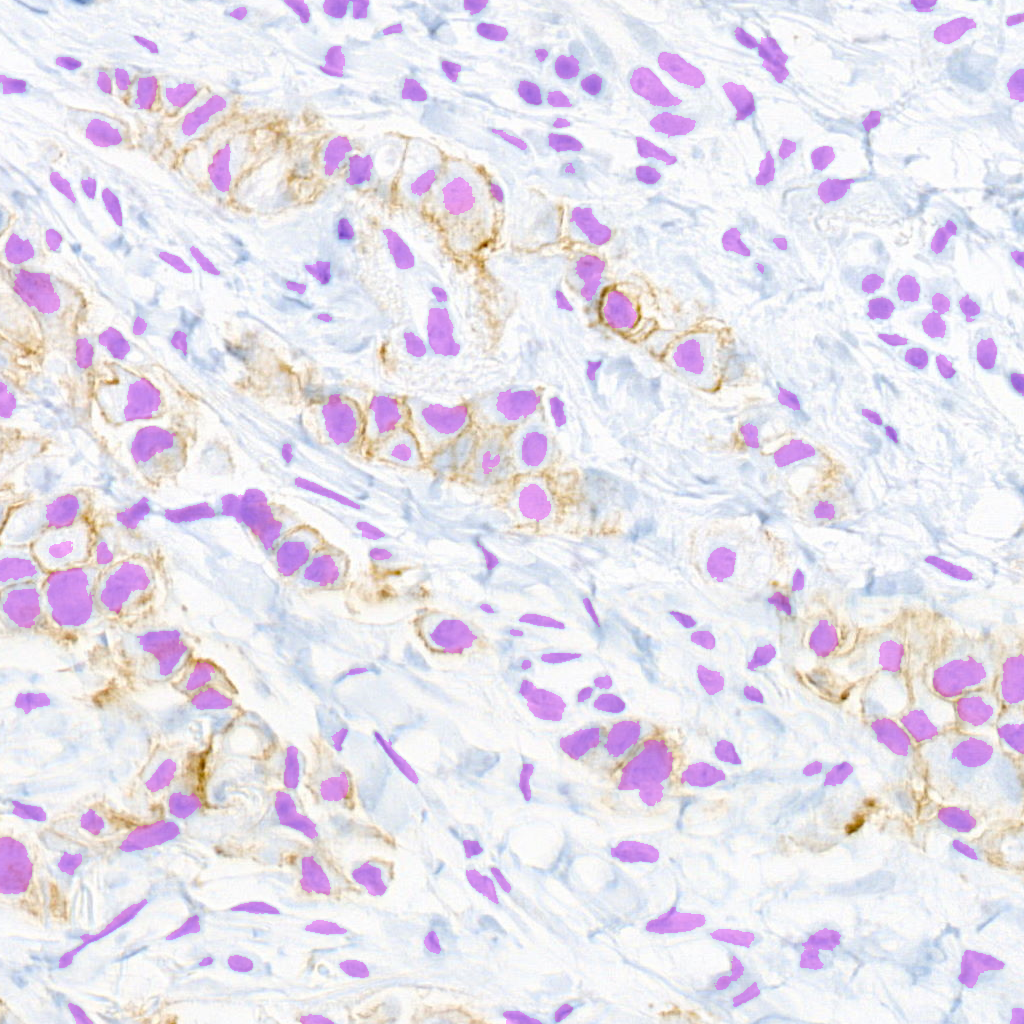
\includegraphics[width=\textwidth]{imgs/qual/breast/void2.png}
    \caption{Void}
    \label{fig:breast-void2}
  \end{subfigure}
  \caption{Illustration of the behaviour of the different models.}
  \label{fig:breast-qual2}
\end{figure}


\begin{figure}[H]
  \centering
  \begin{subfigure}[b]{0.45\textwidth}
    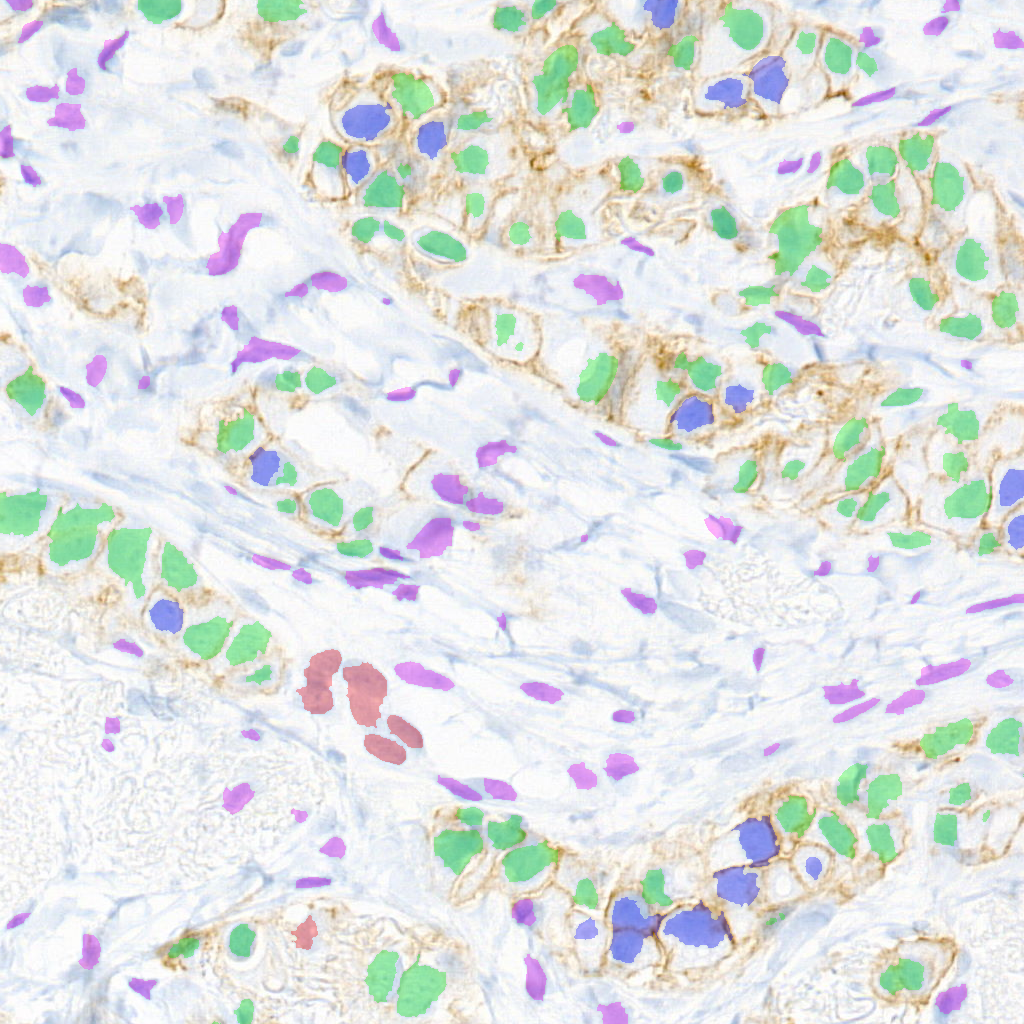
\includegraphics[width=\textwidth]{imgs/qual/breast/gt3.overlay.png}
    \caption{GT}
    \label{fig:breast-gt3}
  \end{subfigure}
  \hfill
  \begin{subfigure}[b]{0.45\textwidth}
    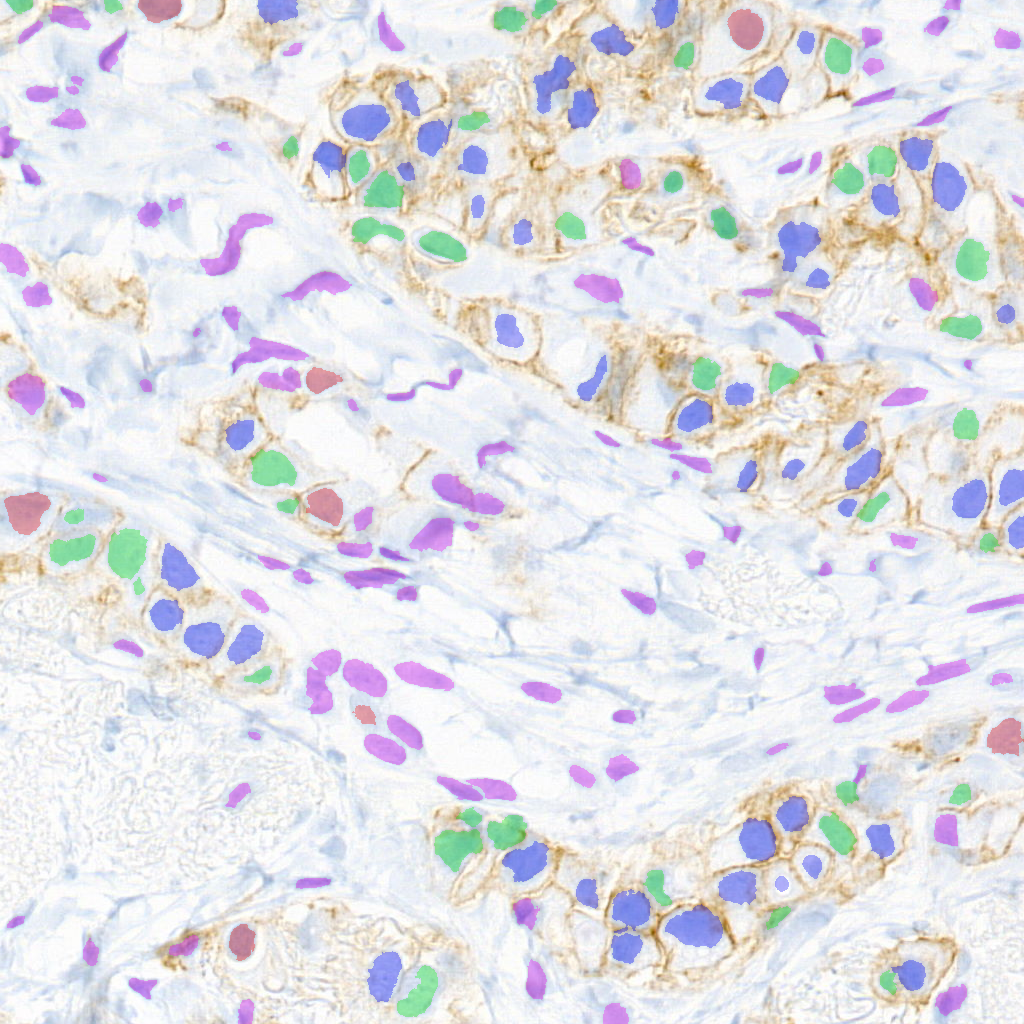
\includegraphics[width=\textwidth]{imgs/qual/breast/hov3.png}
    \caption{Hovernet}
    \label{fig:breast-hov3}
  \end{subfigure}
  \\
  \begin{subfigure}[b]{0.45\textwidth}
    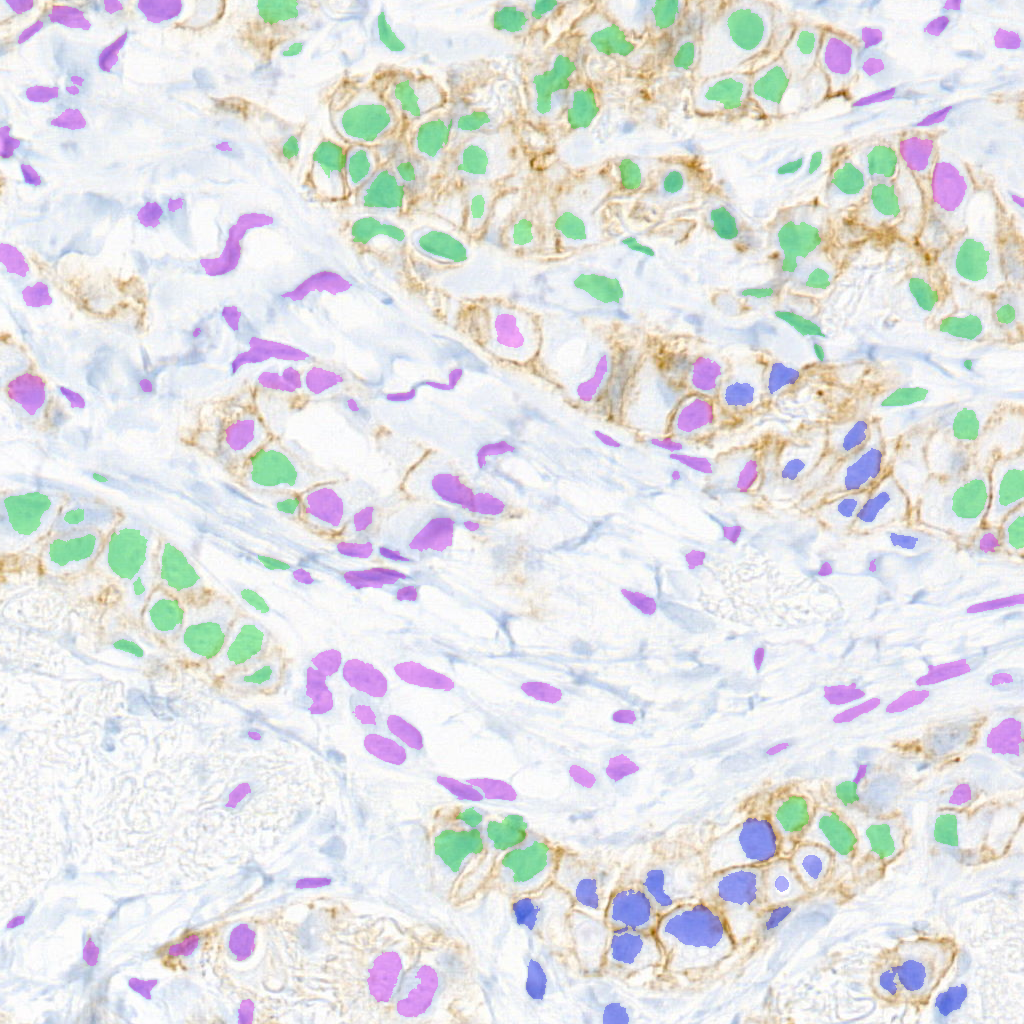
\includegraphics[width=\textwidth]{imgs/qual/breast/gcn-full3.png}
    \caption{GCN}
    \label{fig:breast-gcn3}
  \end{subfigure}
  \hfill
  \begin{subfigure}[b]{0.45\textwidth}
    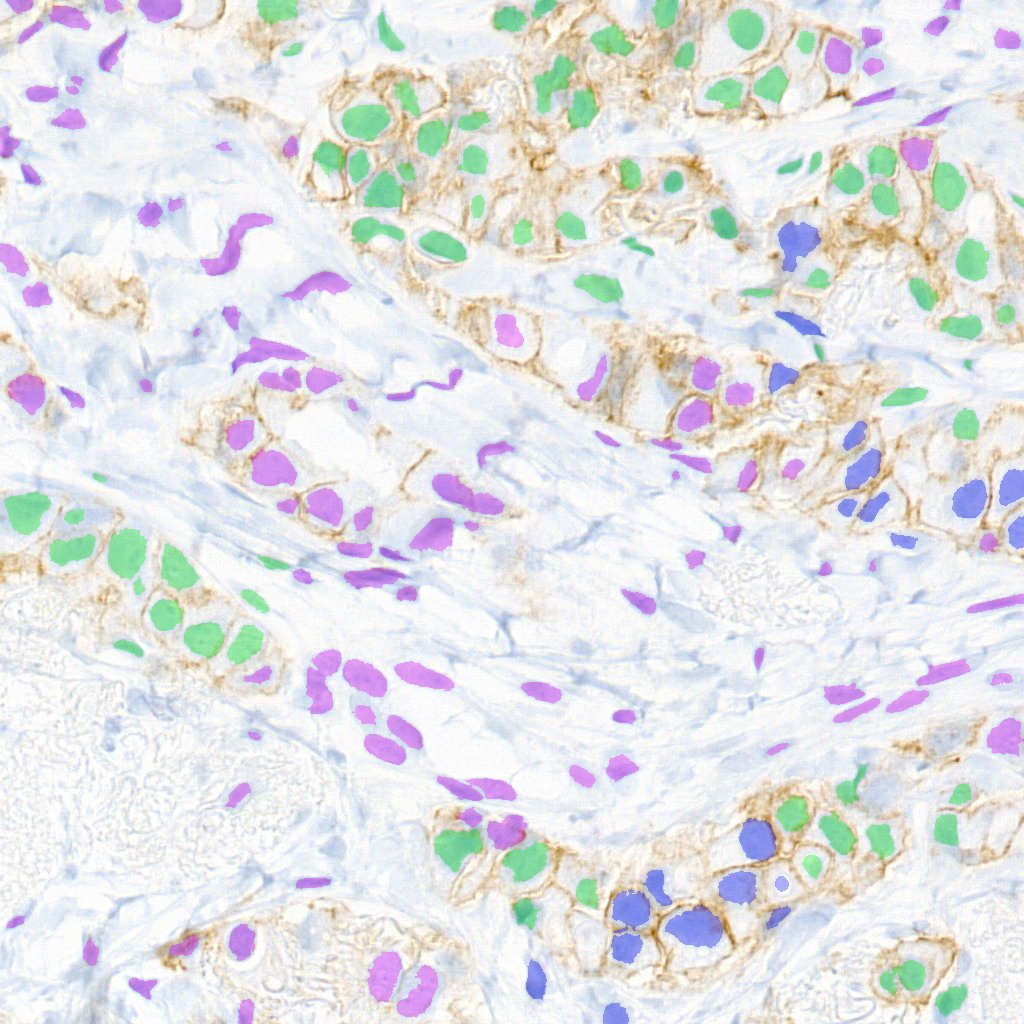
\includegraphics[width=\textwidth]{imgs/qual/breast/no-morph3.png}
    \caption{Probabilities only}
    \label{fig:breast-no-morph3}
  \end{subfigure}
  \\
  \begin{subfigure}[b]{0.45\textwidth}
    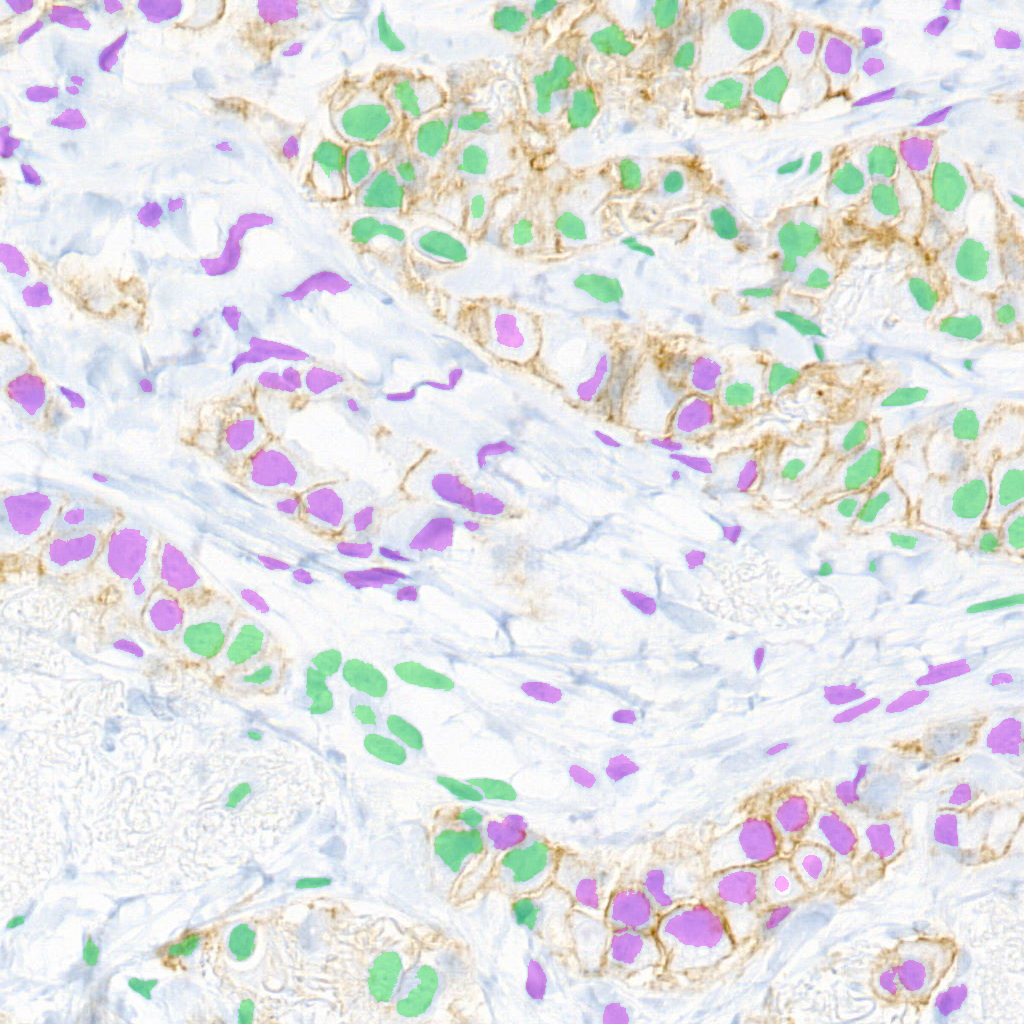
\includegraphics[width=\textwidth]{imgs/qual/breast/no-prior3.png}
    \caption{Morphological features only}
    \label{fig:breast-no-prior3}
  \end{subfigure}
  \hfill
  \begin{subfigure}[b]{0.45\textwidth}
    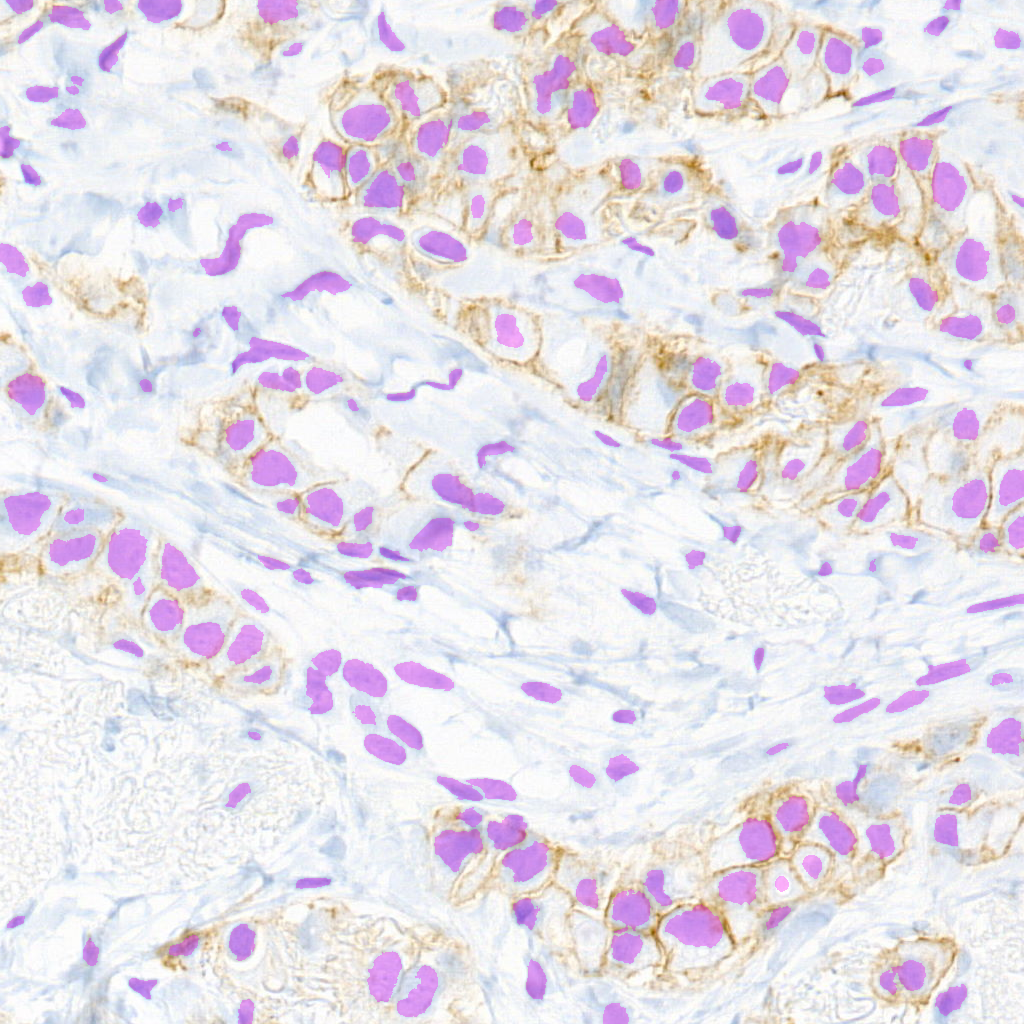
\includegraphics[width=\textwidth]{imgs/qual/breast/void3.png}
    \caption{Void}
    \label{fig:breast-void3}
  \end{subfigure}
  \caption{Yet another illustration of the behaviour of the different models.}
  \label{fig:breast-qual3}
\end{figure}

To finish this section I will compare graph convolution to graph attention. Graph attention networks also create nests of cells. The difference now is that the attention network is trying to detect smaller groups and mixed groups. This may derive from the fact that the attention mechanism gives more flexibility in how labels are propagated through the graph. With the convolution everything gets spread equally likely. But with attention other patterns can emerge and, in fact, emerge. In \autoref{fig:breast-ex2} we can see that in the first pair the graph attention has surrounded a green group by a red group. That is quite unlikely for convolution to do. With the convolution cells get eaten by the biggest group. In the second pair there are some blue cells that are alone in the GAT case and more group diversity. If we consider graph networks to act as regularisers, then GCN penalizes more the existence of lonely cells than GAT.

\begin{figure}[H]
    \centering
    \begin{subfigure}[b]{0.45\textwidth}
    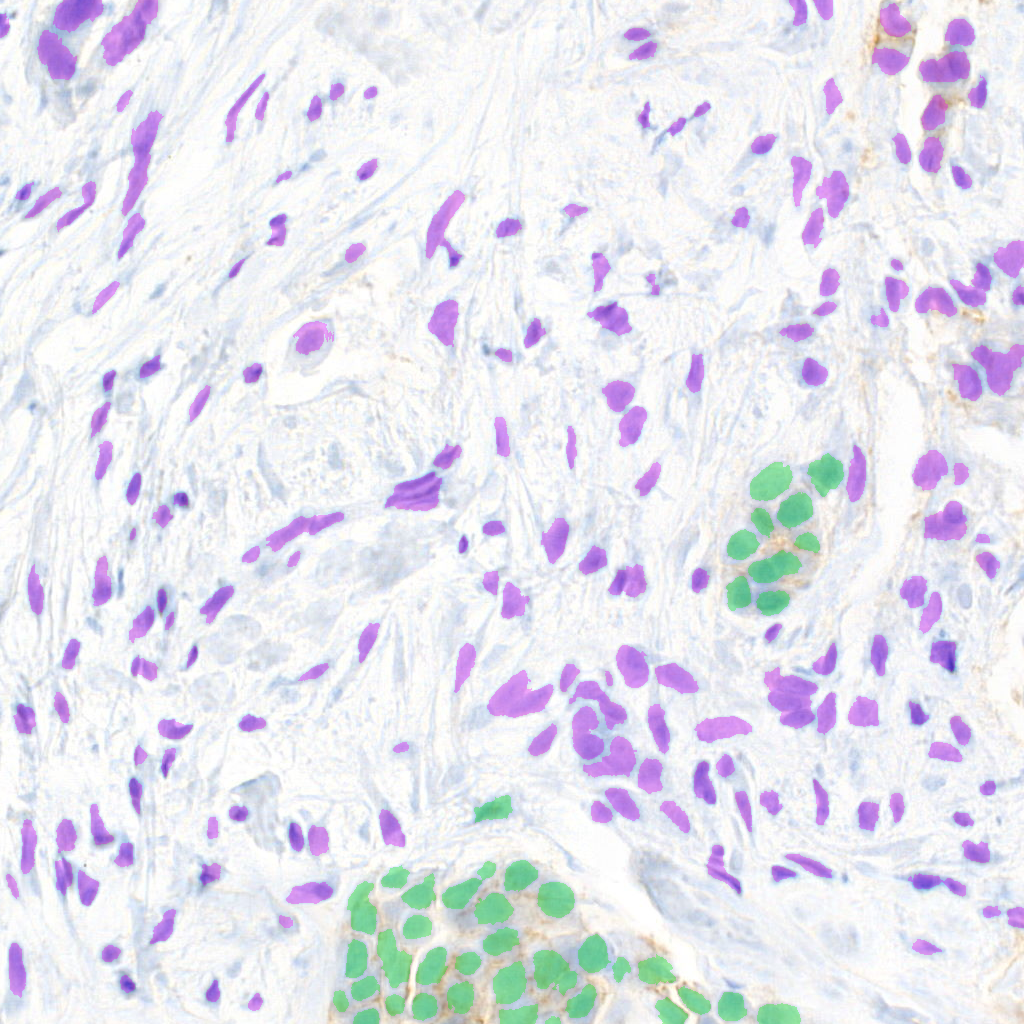
\includegraphics[width=\textwidth]{imgs/qual/breast/gcn-full1.png}
    \caption{GCN}
  \end{subfigure}
  \hfill
  \begin{subfigure}[b]{0.45\textwidth}
    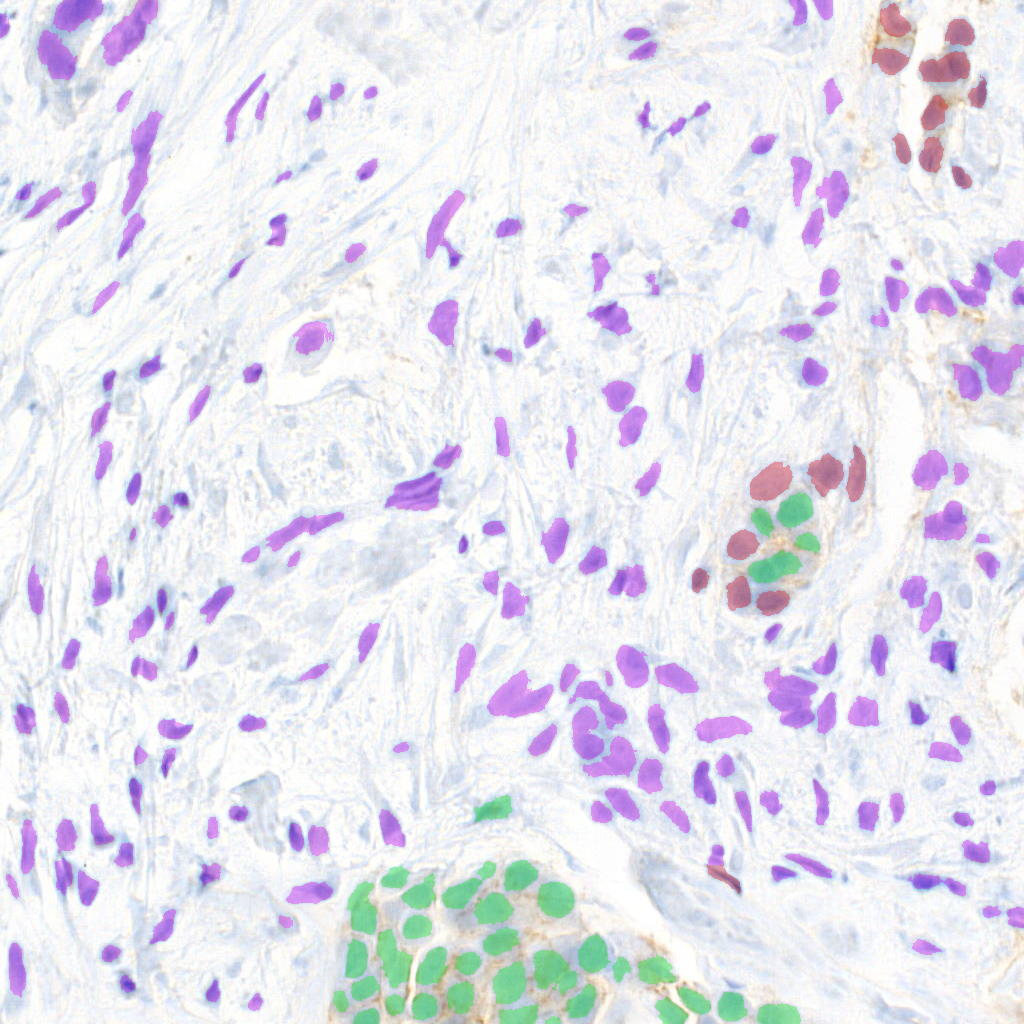
\includegraphics[width=\textwidth]{imgs/qual/breast/gat-full1.png}
    \caption{GAT}
  \end{subfigure}
  \\
  \begin{subfigure}[b]{0.45\textwidth}
    \includegraphics[width=\textwidth]{imgs/qual/breast/gcn-full3.png}
    \caption{GCN}
  \end{subfigure}
  \hfill
  \begin{subfigure}[b]{0.45\textwidth}
    \includegraphics[width=\textwidth]{imgs/qual/breast/gat-full3.png}
    \caption{GAT}
  \end{subfigure}
    \caption{Comparison of graph convolution and graph attention predictions.}
    \label{fig:breast-ex2}
\end{figure}

\newpage
\subsection{DigiPatics lung}

I was personally involved in the creation of this dataset. This means that I know some information that is normally not documented in these databases. When labelling, the physician sometimes decided entirely based on information not present on the image itself. Or information present in the image but very subtle. One such case is the cilium. Cells near cilium are never tumoural but can be very similar to tumoural cells. In all the experiments we made, including those that are not documented here, the specific image in \autoref{fig:lung-cilium} was always predicted as tumoural. However, our best performing graph model somehow solved that problem. It is possible that it has been pure luck. But it is still remarkable because we didn't have such luck with Hovernet.

\begin{figure}[H]
    \centering
    \begin{subfigure}[b]{0.3\textwidth}
    \includegraphics[width=\textwidth]{imgs/qual/lung/cilio-gt.overlay.png}
    \caption{GT}
  \end{subfigure}
  \begin{subfigure}[b]{0.3\textwidth}
    \includegraphics[width=\textwidth]{imgs/qual/lung/cilio-hov.png}
    \caption{Hovernet}
  \end{subfigure}
  \begin{subfigure}[b]{0.3\textwidth}
    \includegraphics[width=\textwidth]{imgs/qual/lung/cilio-no-prior.png}
    \caption{GCN without probabilities}
  \end{subfigure}
    \caption{Example of an image containing cilium together with Hovernet and GNN predictions.}
    \label{fig:lung-cilium}
\end{figure}

Another special case is shown in \autoref{fig:lung-context}. When labelling this specific patch, Irene needed a few minutes to notice that it was not tumoural at all. And she discovered that by looking at the whole slide image. I was told that with that image alone it was not possible to be 100\% sure that all the cells were not tumoural. And we can see that both Hovernet and the GNN fail in this case. The cells marked in blue look so similar to tumoural cells that the models classify them as that because they lack the information needed to discard them from being tumoural.

\begin{figure}[H]
    \centering
    \begin{subfigure}[b]{0.3\textwidth}
    \includegraphics[width=\textwidth]{imgs/qual/lung/context-gt.overlay.png}
    \caption{GT}
  \end{subfigure}
  \begin{subfigure}[b]{0.3\textwidth}
    \includegraphics[width=\textwidth]{imgs/qual/lung/context-hov.png}
    \caption{Hovernet}
  \end{subfigure}
  \begin{subfigure}[b]{0.3\textwidth}
    \includegraphics[width=\textwidth]{imgs/qual/lung/context-no-prior.png}
    \caption{GCN without probabilities}
  \end{subfigure}
    \caption{Example of a patch that required extra context to label together with Hovernet and GNN predictions.}
    \label{fig:lung-context}
\end{figure}
\newpage
To finish this chapter I will leave a canonical example of when graphs are a good fit. The case depicted in \autoref{fig:lung-val} contains three groups perfectly separated from each other. Two nests of tumoural cells at both sides and in the middle a group of healthy cells. Hovernet struggles to detect some of the tumoural cells from the left and right. Probably because they are small, round and with a low nuclei to cytoplasm ratio, which are the properties typical of non-tumoural cells. But they are indeed tumoural, in part because they are all so close together. The graph network, on the other hand, leverages the fact that they are grouped together and propagates the dominant class of each cluster to all the cells of that cluster, perfectly classifying the whole patch.

\begin{figure}[H]
    \centering
    \begin{subfigure}[b]{0.3\textwidth}
    \includegraphics[width=\textwidth]{imgs/qual/lung/val-gt1.overlay.png}
    \caption{GT}
  \end{subfigure}
  \begin{subfigure}[b]{0.3\textwidth}
    \includegraphics[width=\textwidth]{imgs/qual/lung/val-hov1.png}
    \caption{Hovernet}
  \end{subfigure}
  \begin{subfigure}[b]{0.3\textwidth}
    \includegraphics[width=\textwidth]{imgs/qual/lung/val-no-prior1.png}
    \caption{GCN without probabilities}
  \end{subfigure}
    \caption{Another example from the validation dataset where the graph network is clearly better than Hovernet.}
    \label{fig:lung-val}
\end{figure}

